\chapter{Training long short-term memory networks to play the Iterated Prisoner's Dilemma}\label{chapter:lstm}
% TODO another possible title: Machine learning produces successful Iterated Prisoner's Dilemma strategies based on long short-term memory networks

\begin{center}
    The research reported in this Chapter has been carried out with:

    Axerod-Python library version: 4.2.0 \\
    Associated data set: \\ \vspace{.5cm} % TODO archive model weights
\end{center}

\hrulefill

\section{Introduction}

In Chapter~\ref{chapter:meta_tournaments} it was mentioned that consepsualating
and introducing new strategies has been an important aspect of research to the
field. The aim of this Chapter is to introduce new IPD strategies based on an
archetype that has not received much attention in the literature.

In Chapter~\ref{chapter:meta_tournaments} it was concluded that one of the
properties successful strategies in a IPD competition need to have is
cleverness/complexity. Complexity can confer to adaptability, and adaptability
is important in performing well in diverse set of environments. This was
established not only in Chapter~\ref{chapter:meta_tournaments} but also from the
results of Chapter~\ref{chapter:memory_one}. The set of complex strategies that
ranked highly across distinct tournaments in
Chapter~\ref{chapter:meta_tournaments} included strategies based on archetypes
such as finite state automata, hidden Markov models and \textit{artificial
neural networks} (ANNs).

ANNs have successfully been trained to play games exterior to the IPD, such as
checkers~\cite{Chellapilla1999} and chess~\cite{Fogel2004}. The usage of feed
forward ANNs in the IPD was firstly introduced in~\cite{Harrald1996}, and have
been used ever since~\cite{Ashlock2008, Ashlock2006a, Darwen2001, Franken2005}.
Possibly, the most successful ANNs strategies are the one introduced
in~\cite{Harper2017}, as they were ranked \(7^{th}\), \(9^{th}\), and
\(11^{th}\) in a tournament of 223 strategies.

A type of ANNs that have not received much attention in the literature are the
\textit{recurrent neural networks} (RNNs). RNNs are a type of neural networks
that include a feedback connection and are designed to work with inputs in
the form of sequences. RNNs were firstly considered as an archetype in 1996.
In~\cite{Sandholm1996} a RNN which considered a single previous step
as an input was trained via a \(Q\) learning algorithm to play against a single
strategy. The results of~\cite{Sandholm1996} were limited only in the network
learning to play against a single strategy.

The limitations of~\cite{Sandholm1996} could potentially have been due to the
limitations of the RNNs themselves. As it will be discussed later the RNNs
quickly became unable to learn due to the vanishing gradient problem.
To improve on the standard recurrent networks a new network called the
long short-term memory networks (LSTMs) were introduced in~\cite{Hochreiter1997}.
LSTMs do not suffer from the vanishing gradient, can be successfully trained and
are being used in a number of innovative applications such as time series analysis
\cite{Malhotra2015}, speech recognition~\cite{Sak2014} and prediction in
medical care pathways~\cite{Wang2018_lstm}.

LSTMs have not received attention in the IPD literature. This Chapter trains and
introduced a number of strategies  based on LSTMs. The training has been
possible due to the collection of best response sequences generated in
Chapter~\ref{chapter:best_response_sequence}. The performance of the new
strategies is evaluated and compared in a meta tournament analysis of standard
tournaments. The results demonstrate % TODO add results

This Chapter is structured as follows:

\begin{itemize}
    \item section~\ref{section:artificial_neural_networks}, presents an
    introduction to artificial, recurrent and long short-term memory networks.
    \item section~\ref{section:training_a_rnn}, cover the specifics of the LSTMs
    trained in ths Chapter. Their architectural details are presented as well as
    the different training sets they have been trained on.
    \item section~\ref{section:rnn_strategy_validation}, evaluates and compares
    the performance of \lstmstrategies LSTMs based strategies in
    \metatournamentslstm standard IPD computer tournaments.
\end{itemize}

\section{Artificial, recurrent neural and long short-term memory networks}\label{section:artificial_neural_networks}

ANNs are computing systems vaguely inspired by the biological neural networks
that constitute animal brains. As stated in~\cite{Jain1996} the research on ANNs
has experienced three periods of extensive activity. The first peak was in the
1940s. The work of~\cite{McCulloch1943} opened the subject by creating a
computational model for neural networks. The second peak occurred in 1960s with
the introduction of the perceptron~\cite{Rosenblatt1958}. The perceptron is a
linear binary classifier and in the 1960s in was shown that it could be used to
learn to classify simple shapes with \(20\times20\) pixels input. However, it
was impossible for the perceptron to be extended to classification tasks with
many categories. The limitations of the model were presented
in~\cite{Minsky1969} which alted the enthusiasm of most researchers in ANNs,
resulting in no activity in field for almost 20 years. The third peak occurred
in the early 1980s with the introduction of the back propagation algorithm for
multilayered networks~\cite{Werbos1974}. Though the algorithm was initially
proposed by~\cite{Werbos1974} it has been reinvented several times and it was
popularizes by~\cite{McClelland1986}. Following the introduction of the
algorithm and the ability to now train more complex models, ANNs have received
considerable interest, and have been used in a number of innovative applications
such as \cite{Covington2016, Kalogirou2000}.

ANNs based on the connection pattern/architecture can be grouped into two
categories:

\begin{itemize}
    \item Feed forward networks.
    \item Recurrent or feedback networks.
\end{itemize}

ANNs can be viewed as weighted directed graphs in which artificial neurons are
nodes and directed edges, with weights, are connections between the neuron
outputs and the neuron inputs~\cite{Jain1996}. In feed forward networks the
graphs have no loops whereas in recurrent loops occur because of feedback
connections. A graphical representation of a feed forward network with a single
hidden layer is given by Figure~\ref{fig:ann}.

\begin{figure}[!htbp]
    \centering
    \includestandalone[width=.5\textwidth]{src/chapters/07/neural_network}
    \caption{Graphical representation of an ANN.}\label{fig:ann}
\end{figure}

A feed forward network is composed by an input layer, hidden layers, and an
output layer. The networks' input is a vector \(x\). The dimensionality, or
number of nodes of the input layer is depended on the dimensionality of \(x\).
Each element of the input vector is connected to the hidden layer via a set of
learned weights. The hidden layer also consists of nodes and the number of
node/dimensionality of it is an architectural decision. The \(j^{\text{th}}\)
hidden neuron outputs,

\[h_j = \phi (\sum_{i} w_{ij} x_{i}), \text{where } \phi  \text{ is an activation function}.\]

Common activation functions for \(\phi\) include:

\begin{itemize}
    \item the sigmoid function \(\sigma(x)\) which squashes numbers into the range \([0, 1]\)
    \item the hyperbolic tangent, \(tanh(x)\) which squashes numbers into the range \([-1, 1]\)
    \item the rectified linear unit, \(ReLU(x)=max(0,x)\)
\end{itemize}

In turn, the hidden layer is fully connected to an output layer. The
\(j^{\text{th}}\) output neuron outputs,

\[y_{j} = \sum_{i} v_{ij} h_{i}.\]

The output layer transforms the raw scores to probabilities via a softmax function.

Feed forward networks make predictions using forward propagation,

\begin{align}\label{eq:neural_network_equations}
h & = \phi(Wx) \\ \label{eq:neural_network_equations_two}
y & = \text{softmax}(Vh)
\end{align}

where \(W\) is a weight matrix connecting the input and hidden layers, \(V\) is
a weight matrix connecting the hidden and output layers. \(W\) and \(V\) are the
learning parameters of the network. Their dimensionality depends on the
dimensionality of networks layers. If \(x\) and \(x\) are  2 dimensional and the
hidden layer had 500 nodes then \(W \in \R^{2 \times 200}\) and \(V \in \R^{2
\times 200}\). Increasing the dimensionality of the hidden layer corresponds to
more parameters.

Training a ANN corresponds to finding the learning parameters that minimise
the error on the training data. The function that measures error is called
the \textit{loss function}. A common loss function with the choice of
a softmax output is the \textit{cross entropy} loss. Consider \(N\) training
examples and \(K\) classes, the function for a prediction \(\hat{y}\) with
respect to the true output \(y\) us give by,

\[L(y, \hat{y}) = - \frac{1}{N} \sum_{n\in N} \sum_{k \in K} y_{n, k} \text{log}(\hat{y_{n, k}})\]

The minimum of the loss function is calculated using the gradients decent
algorithm. The gradient decent algorithm relies on the gradients. The gradients
are the vector of derivatives of the loss function with respect to the learning
parameters. Thus, \(\frac{\partial{L}}{\partial{W}}\) and
\(\frac{\partial{L}}{\partial{V}}\). These gradients are calculated with the
back propagation algorithm~\cite{Wythoff1993}, which is a way to efficiently
calculate the gradients starting from the output.

An extension of feed forward networks are the recurrent networks. RNNs are
capable of processing variable length sequences of inputs. More importantly,
RNNs use their internal state/knowledge to a make a prediction on the input at
time \(t\) based on the decisions made at the previous time steps. A graphical
representation of a RNN is given by Figure~\ref{fig:rnn}. RNN are networks with
loops. The loop represents that information can be passed down from one step of
the network to the next. In fact they can be thought of as multiple copies of
the same network, each passing a message to a successor, as demonstrated by
Figure~\ref{fig:rnn}.

\begin{figure}[!htbp]
    \centering
    \includestandalone[width=\textwidth]{src/chapters/07/reccurent_neural_network}
    \caption{Graphical representation of a RNN.}\label{fig:rnn}
\end{figure}

The hidden layers pass down information by considering,

\begin{equation*}
    h_t = \phi(Wx_t + Uh_{t-1})
\end{equation*}

where \(h_{t-1}\) is the hidden state computed at time \(t-1\) multiplied by
some weight vector \(U\). In matrix notation RNNs are described by,

\begin{align}\label{eq:recurrent_neural_network_equations}
    h_t & = \phi(Wx_t + Uh_{t-1}) \\
    y_t & = Vh
\end{align}

Unfortunately, in practice RNNs quickly become unable to learn to connect the
information. The more time steps the higher the chance that the back propagation
gradient either accumulate and explode or vanish down to zero. The fundamental
difficulties of RNNs were explored in depth by~\cite{Bengio1994}.

A network specifically designed to avoid the long-term dependency problem. was
introduced by~\cite{Hochreiter1997} called the long short-term memory network
(LSTM). LSTMs work tremendously well on a large variety of problems, and are now
widely used. Remembering information for long periods of time is practically
their default behavior, not something they struggle to learn.

The core idea to LSTMs is the \textit{cell state} also refereed to as the
long term memory, denote as \(C_t\). The cell state is designed to pass down
information with only a few carefully regulated changes being applied to it
by structures called \textit{gates}. Gates are composed out of a sigmoid neural
net layer and a point wise multiplication operator. In order to explain
the cell gate and subsequently how LSTMs make predictions consider
a LSTM's hidden layer at time step \(t\) give by Figure~\ref{fig:lstm_cell}.

\begin{figure}[!htbp]
    \centering
    \includestandalone[width=.7\textwidth]{src/chapters/07/lstm_cell}
    \caption{An LSTM hidden layer at time step \(t\).}\label{fig:lstm_cell}
\end{figure}

The cell state and hidden state from from the previous time step are feed back
into the network. Initially, the network decides what information from the
previous cell state is to be discarded. This decision is made by the
\textit{forget state}. The forget state considers the hidden state at time
\(t-1\) and the input at time \(t\),

\begin{equation}\label{eq:forget_gate}
    f_{t} = \sigma(W_{f}x_{t} + U_{f}h_{t-1})
\end{equation}

Secondly, the network decides what information is going to be stored at the
cell gate. There are two parts to this. Firstly, the input gate decides which values
are going to be updated,

\begin{equation}\label{eq:input_gate}
    i_{t} = \sigma(W_{i}x_{t} + U_{i}h_{t-1} + b_{i}).
\end{equation}

and secondly, a tanh layer creates a vector of candidate values denoted as
\(\tilde{C}_{t}\) that could be added to the cell state. \(\tilde{C}_{t}\) 
is given by Equation~(\ref{eq:input_gate}).

\begin{equation}\label{eq:input_gate}
    \tilde{C}_{t} = tanh(W_{c}x_{t} + U_{c}h_{t-1} + b_{c}).
\end{equation}

The cell state \(C_{t-1}\) is multiplied by \(f_{t}\), forgetting the values
which have been decided to discard. The new candidate values are scaled by how
much information has been decided to keep from the input. Thus,

\begin{equation}\label{eq:input_gate}
    C_{t} = f_{t} * C_{t-1} + i_{t} * \tilde{C}_{t}.
\end{equation}

The LSTM outputs a hidden state at each time step. This is either used to
through an activation function to output \(y_{t}\), and it is passed to the next
time step cell. The output is based on the current cell state. The cell state
goes through a tanh function and it is multiplied by a sigmoid gate that decides
which parts to output from the cell state.

\begin{align}\label{eq:input_gate}
    o_{t} & = \sigma(W_{o}x_{t} + U_{o}h_{t-1} + b_{o}), \\
    h_{t} & = o_{t} * tanh(C_{t})
\end{align}

This process is being carried out though each time step of the input sequence.
At each the cell state and hidden state are feed back into the network and the
hidden state can also be used to make a prediction for each time step as
demonstrated by Figure~\ref{fig:lstm}.

\begin{figure}[!htbp]
    \centering
    \includestandalone[width=\textwidth]{src/chapters/07/lstm}
    \caption{Graphical representation of an LSTM network.}\label{fig:lstm}
\end{figure}

The LSTM is a complex architecture and contains a large number of parameters
that need to be trained. The LSTM networks have managed to achieve remarkable
results. The training of an LSTM model in this Chapter is carried with the open
source project Keras. The details for the training are presented in
section~\ref{section:training_a_rnn}.

\section{Training LSTM networks to play the Iterated Prisoner's Dilemma}\label{section:training_a_rnn}

LSTM are trained in a supervised fashion on a set of training sequences. The
purpose of training a network in this Chapter is so it can learn to play the
IPD. For that reason the networks are going to be trained on the collection of
best response sequences generated in
Chapter~\ref{chapter:best_response_sequences}. The collection was purposely generated
so that the networks could be trained to play optimal against a list of known
IPD strategies.

The inputs of a network are the actions of a given strategy and the expected
output is the response of the best response sequence to that action. More
specifically, each pair of opponent's - best response sequence's actions
correspond to 204 training inputs with a maximum dimensionality of 204.

Consider the actions of the strategy Adaptive and a best response to it as
presented in section~\ref{section:the_collection_of_best_response_sequences}
given by Table~\ref{table:adaptive_vs_best_response_binary_lstm}.

\begin{table}[htbp]
    \centering
    \begin{tabular}{cccccccccccccccc}
        & \textbf{1} & \textbf{2} & \textbf{3} & \textbf{4}  & \textbf{5} & \textbf{6} & \textbf{7} & \textbf{8} & \textbf{9} & \textbf{10} & \textbf{11} &  \textbf{12} & \(\dots\)  & \textbf{204} &  \textbf{205} \\ 
        \midrule
        Adaptive & 1 & 1 & 1 & 1 & 1 & 1 & 1 & 0 & 0 & 0 & 0& 1& \(\dots\) & 1 & 1 \\
        \(S^*\) & 1 & 1 & 0 & 0 & 0 & 0 & 0 & 0 & 0 & 0 & 0 & 0& \(\dots\) & 0 & 0 \\ \bottomrule
    \end{tabular}
    \caption{The actions of the strategy Adaptive against one of the best response sequences
    to the strategy. Note that \(0 \to D\) and \(1 \to C\).}\label{table:adaptive_vs_best_response_binary_lstm}
\end{table}

The highest dimensionality the input vector \(x\) to the network can have is
204. This is because the expected output of to Adaptive's action in turn 1 is
the action of the best response sequence at turn 2. Moreover, the expected
output to the Adaptive's \(204^{\text{th}}\) action is the best response's
\(205^{\text{th}}\) action. This is demonstrated by
Figure~\ref{fig:input_output_example}.

\begin{figure}[!htbp]
    \centering
    \includestandalone[width=\textwidth]{src/chapters/07/output}
    \caption{An example of a networks input and output of \(t=204\). The last
    action of Adaptive as well as the first action of the best
    response sequence are discarded.}\label{fig:input_output_example}
\end{figure}

The networks of this Chapter have been trained for a non fixed sequence length.
In order to train the networks on different input lengths each pair opponent's -
best response sequence's actions is broken down to 204 distinct inputs. This is
done so that each input captures the play of 204 IPD matches between the pairs
where the number of turns \(N \in [1, 204]\). For example the training points
from Table~\ref{table:adaptive_vs_best_response_binary_lstm} are given by,

\begin{equation}\label{eq:sequence_to_sequence_inputs_outputs_example}
    \text{inputs} =
    \begin{bmatrix}
        1 &  &  \\
        1 & 1 &  \\
        1 & 1 & 1 \\
        1 & 1 & 1 & 1 \\
        1 & 1 & 1 & 1 & 1 \\
        1 & 1 & 1 & 1 & 1 & 1\\
        1 & 1 & 1 & 1 & 1 & 1 & 0 \\
        \vdots & \vdots & \vdots & \vdots & \vdots & \vdots & \vdots \\
    \end{bmatrix}
    \text{expected outputs} =
    \begin{bmatrix}
        1 &  &  \\
        1 & 1 &  \\
        1 & 1 & 0 \\
        1 & 1 & 0 & 0 \\
        1 & 1 & 0 & 0 & 0 \\
        1 & 1 & 0 & 0 & 0 & 0\\
        1 & 1 & 0 & 0 & 0 & 0 & 0 \\
        \vdots & \vdots & \vdots & \vdots & \vdots & \vdots & \vdots \\
    \end{bmatrix}
\end{equation}

Thus the training data set created by the best response collection correspond
to \(\totalsequences \times 204 = \trainingpoint\) training inputs.

Two variants of LSTMs have been trained in this Chapter. These are refereed to:

\begin{itemize}
    \item sequence to sequence
    \item sequence to probability
\end{itemize}

The sequence to sequence model as an input of actions a each time step by a
strategy an it outputs a response for each at each time step. The sequence to
probability has an input the action of strategy up to time \(t\), and outputs a
response to the history at time \(t\). Both networks output a probability which
is translated at the probability of cooperating after the opponent's last \(t\)
actions. A graphical representation of the two networks are given by
Figures~\ref{fig:sequence_to_sequence} and \ref{fig:sequence_to_probability}.

\begin{figure}[!htbp]
    \centering
    \includestandalone[width=\textwidth]{src/chapters/07/sequence_to_sequence}
    \caption{A graphical representation of a sequence to sequence LSTM model}.\label{fig:sequence_to_sequence}
\end{figure}

\begin{figure}[!htbp]
    \centering
    \includestandalone[width=\textwidth]{src/chapters/07/sequence_to_probability}
    \caption{A graphical representation of a sequence to probability LSTM model}.\label{fig:sequence_to_probability}
\end{figure}

The training data of the sequence to sequence model is the form of
Equation~(\ref{eq:sequence_to_sequence_inputs_outputs_example}) whereas the
training data for the sequence to probability model are in the form of
Equation~(\ref{eq:sequence_to_probability_inputs_outputs_example}).

\begin{equation}\label{eq:sequence_to_probability_inputs_outputs_example}
    \text{inputs} =
    \begin{bmatrix}
        1 &  &  \\
        1 & 1 &  \\
        1 & 1 & 1 \\
        1 & 1 & 1 & 1 \\
        1 & 1 & 1 & 1 & 1 \\
        1 & 1 & 1 & 1 & 1 & 1\\
        1 & 1 & 1 & 1 & 1 & 1 & 0 \\
        \vdots & \vdots & \vdots & \vdots & \vdots & \vdots & \vdots \\
    \end{bmatrix}
    \text{expected output} =
    \begin{bmatrix}
        1 \\
        1 \\
        0 \\
        0 \\
        0 \\
        0 \\
        0 \\
        \vdots \\
    \end{bmatrix}
\end{equation}

\subsection{Building the networks with Keras}

The open source neural-network package Keras~\cite{Chollet2015} is used to
construct and train the networks. Keras is a library written in Python designed
to enable fast experimentation with neural networks. Neural layers, cost
functions, optimizers and activation functions are all standalone modules that
can be combined to create new network models.

The Python code for implementing the sequence to sequence model is given by
Figure~\ref{fig:keras_sequence_to_sequence}. In line 12 the model is defined to
be of the \mintinline{python}{Sequential} class. This mean that the model will
constructed layer by layer. The sequence to sequence network has a single LSTM
layer with 100 nodes. The input to the LSTM network is not a fixed length
and there a single time step between the elements of each input sequence.
Those are defined by the argument \mintinline{python}{input_shape=(None, 1)}.
The LSTM layer outputs the hidden states at each time step and they go through
a dropout layer then are transformed into an a probability output via a
sigmoid layer. There are a total of 41301 learning parameters to the sequence
to sequence model.

\begin{figure}[!htbp]
\begin{usagepy}
>>> from keras.models import Sequential

>>> from keras.layers import (
...     Dense,
...     Dropout,
...     CuDNNLSTM,
... )

>>> num_hidden_cells = 100
>>> drop_out_rate = 0.2

>>> model = Sequential()

>>> model.add(
...    CuDNNLSTM(
...        num_hidden_cells, return_sequences=True, input_shape=(None, 1))
...)

>>> model.add(Dropout(rate=drop_out_rate))

>>> model.add(Dense(1, activation="sigmoid"))
>>> model.summary()
Model: "sequential_1"
_________________________________________________________________
Layer (type)                 Output Shape              Param #   
=================================================================
cu_dnnlstm_1 (CuDNNLSTM)     (None, None, 100)         41200     
_________________________________________________________________
dropout_1 (Dropout)          (None, None, 100)         0         
_________________________________________________________________
dense_1 (Dense)              (None, None, 1)           101       
=================================================================
Total params: 41,301
Trainable params: 41,301
Non-trainable params: 0
_________________________________________________________________

\end{usagepy}
\caption{Python code for implementing the sequence to sequence LSTM with Keras.}\label{fig:keras_sequence_to_sequence}
\end{figure}

Regarding the dimensionality of the hidden layer there is no direct answer as to
what is the optimal number of nodes. Several methods for determining the
dimensionality include experimentation, intuition and examples of other trained
networks. Trained networks and tutorial have suggested that using a number
smaller than the maximum sequence length and around a 100 is a good value. As
with all machine learning over fitting is an issue that can occur during
training. A simple and yet efficient method to reduce over fitting is randomly
dropping out nodes during training. That is the usage of the dropout layer.

The Python code for implementing the sequence to probability network with Keras
is given by Figure~\ref{fig:keras_sequence_to_probability}. The implementations
of the networks are similar, however, the sequence to probability model contains
2 LSTM layers. The first LSTM layer outputs the hidden states at each time steps
and these are feed to the second layer which only output the hidden state at
final time step. The output of the network is a probability. The sequence to
probability network has a higher number of learning parameters due to the two
LSTM layers. More specifically, there are 122101 learning parameters to the
network.

\begin{figure}[!htbp]
\begin{usagepy}
    >>> from keras.models import Sequential
>>> from keras.layers import (
...     Dense,
...     Dropout,
...     CuDNNLSTM,
... )

>>> num_hidden_cells = 100
>>> drop_out_rate = 0.2

>>> model = Sequential()

>>> model.add(
...     CuDNNLSTM(num_hidden_cells, return_sequences=True, input_shape=(None, 1))
... )

>>> model.add(CuDNNLSTM(num_hidden_cells))
>>> model.add(Dropout(rate=drop_out_rate))

>>> model.add((Dense(1, activation="sigmoid")))
>>> model.summary()
Model: "sequential_2"
_________________________________________________________________
Layer (type)                 Output Shape              Param #   
=================================================================
cu_dnnlstm_2 (CuDNNLSTM)     (None, None, 100)         41200     
_________________________________________________________________
cu_dnnlstm_3 (CuDNNLSTM)     (None, 100)               80800     
_________________________________________________________________
dropout_2 (Dropout)          (None, 100)               0         
_________________________________________________________________
dense_2 (Dense)              (None, 1)                 101       
=================================================================
Total params: 122,101
Trainable params: 122,101
Non-trainable params: 0
_________________________________________________________________

\end{usagepy}
\caption{Python code for implementing the sequence to probability LSTM with Keras.}\label{fig:keras_sequence_to_probability}
\end{figure}

Keras includes two implementations for an LSTM layer. The class
\mintinline{python}{LSTM} and the class \mintinline{python}{CCNLSTM} which is
the class used here. \mintinline{python}{CCNLSTM} provides a faster
implementation of \mintinline{python}{LSTM} the NVIDIA CUDA Deep Neural Network
library. The \mintinline{python}{CCNLSTM} class allows the networks to be
trained on a graphics processing unit (GPU).

\subsection{Training on GPU}

Conventionally executing computer code happens on the central processing unit
(CPU). The CPU, also called main processor, is essentially the brain of any
computing device. Architecturally the CPU is composed of just a few cores
designed to support an extremely broad variety of tasks.

A graphical processing unit (GPU), on the other hand, is composed of hundred of
cores designed to process a set of simpler and more identical computations in
parallel. GPUs were initially designed as dedicated graphical rendering
workhorses of computer games but ere later enhanced to accelerate other
geometric calculations. NVIDIA created a parallel computing architecture and
platform for its GPUs called CUDA, which gave developers access and the ability
to express simple processing operations in parallel through code.

While a CPU core is more powerful than a GPU core, the vast majority of this
power goes unused by machine learning applications. A GPU core is optimised
exclusively for data computations and because of this singular focus, a GPU core
is simpler and has a smaller die area than a CPU, allowing many more GPU cores
to be crammed onto a single chip. Consequently, machine learning applications,
which perform large numbers of computations on a vast amount of data, can see
huge performance improvements when running on a GPU versus a CPU.

The training process of the LSTM networks here is carried out on a GPU. More
specifically, the training process was carried out on the High-Performance
Computing (HPC) cluster of Cardiff University.

\subsection{Training data sets}

It was explained in the the best response data set from Chapter 6 is used as
training data. Moreover, each best responses has broken down to 204 different
inputs. In order to understand the difference the effect of the training data
the models have been trained on different subsets of the data set. More
specifically in total of four different sub sets. These with a brief explanation
and number are given by Table~\ref{table:training_data_sets}.

\newcolumntype{g}{>{\columncolor{Gray}}c}
\begin{table}[htb]
    \centering
    \resizebox{\textwidth}{!}{
    \begin{tabular}{cglg}
    \toprule
    Data set & number of \(Q\) & Explanation & number of \(S^*\) \\
    \midrule
    all strategies & \numberofstrategiesbestsequences & The data set as presented in Chapter~\ref{chapter:best_response_sequence} & \totalsequences \\
    top performing strategies & \topstrategies & Top \topstrategies performing strategies in a standard tournaments performed with APL & \topsequences \\
    strategies across ranks & \acrossstrategies & A set \acrossstrategies that there rank is across & \acrosssequences\\
    basic strategies & \basicstrategies & A set \basicstrategies which are classified as the basic in APL & \basicsequences \\ 
    \bottomrule
    \end{tabular}}
    \caption{Subset of data set that the networks are trained on. The APL project
    performs a round robin tournament with all the strategies implemented on every release.
    The top strategies and the strategies across are based on the results of the tournament
    with APL version 4.5.0.}\label{table:training_data_sets}
\end{table}

Due to the different size of the data set the networks have trained for a different
number of epochs. The number of epochs is the number of complete passes through
the training data set. The number of epochs each network has trained for each
data set is given by Table~\ref{table:epochs}.

\begin{table}[!htbp]
    \begin{center}
    \resizebox{.9\textwidth}{!}{
        \begin{tabular}{lcccc}
\toprule
{} &  all strategies &  top strategies &  strategies across ranks &  basic strategies \\
\midrule
sequence to sequence    &           19999 &           83999 &                    39999 &            129999 \\
sequence to probability &            7999 &           74999 &                    39999 &             84999 \\
\bottomrule
\end{tabular}

    }
\end{center}
\caption{Number of epochs each both networks, sequence to sequence and 
sequence to probability, were trained for each subset.}\label{table:epochs}
\end{table}

The data are split into training and test training set. The test set is
20\% of the data. The validation and loss is calculated at each epoch.
The validation is the measure that. The loss is based on the.


\begin{figure}[!htbp]
    \begin{subfigure}{\textwidth}
    \centering
    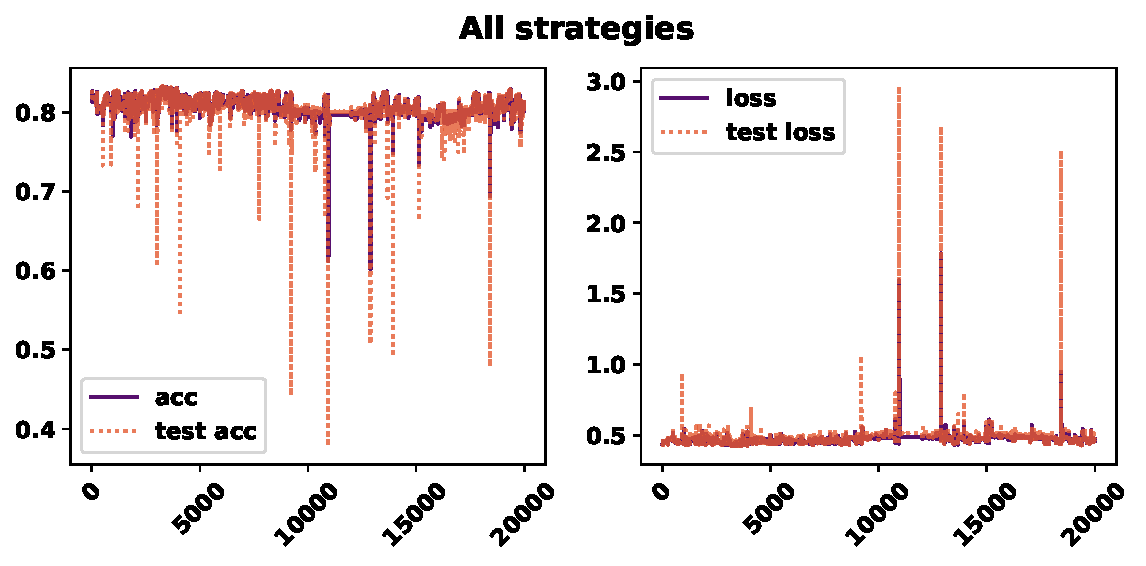
\includegraphics[width=.8\textwidth]{src/chapters/07/img/validation_plot_all_strategies.pdf}
    \end{subfigure}\hfill
    \begin{subfigure}{\textwidth}
    \centering
    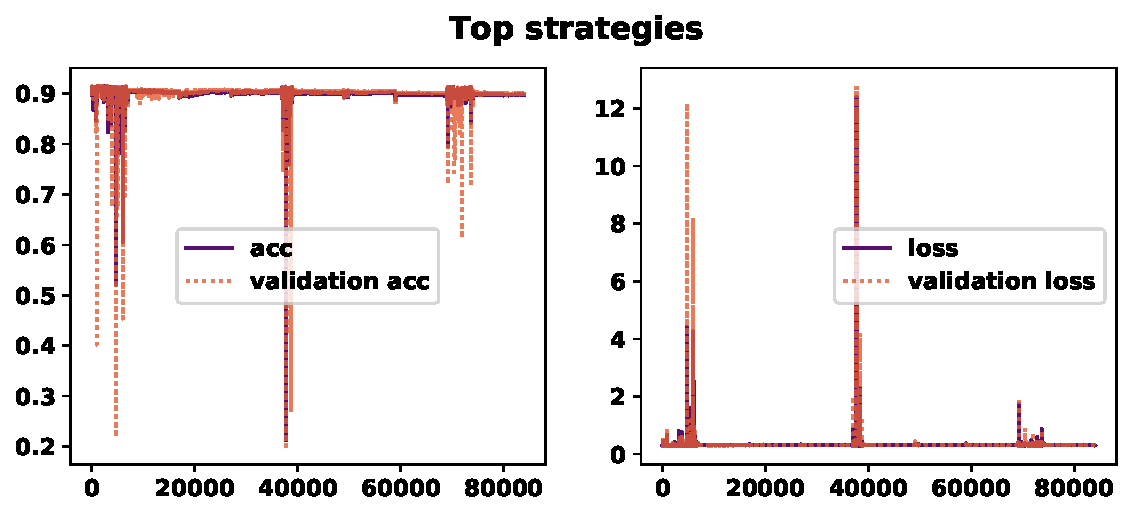
\includegraphics[width=.8\textwidth]{src/chapters/07/img/validation_plot_top_strategies.pdf}
    \end{subfigure}
    \begin{subfigure}{\textwidth}
    \centering
    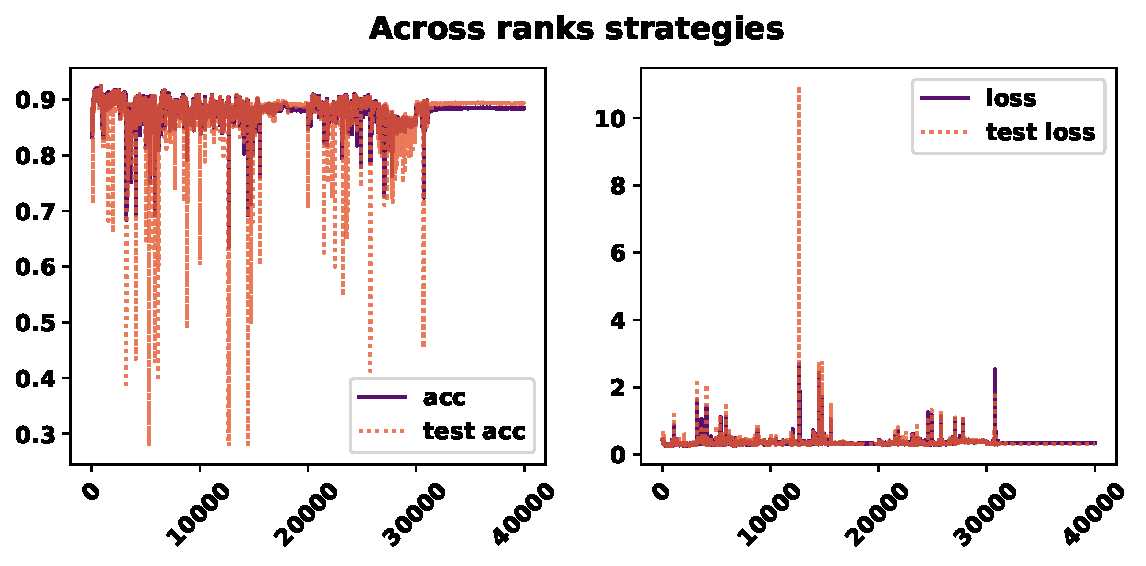
\includegraphics[width=.8\textwidth]{src/chapters/07/img/validation_plot_across_ranks_strategies.pdf}
    \end{subfigure}
    \begin{subfigure}{\textwidth}
    \centering
    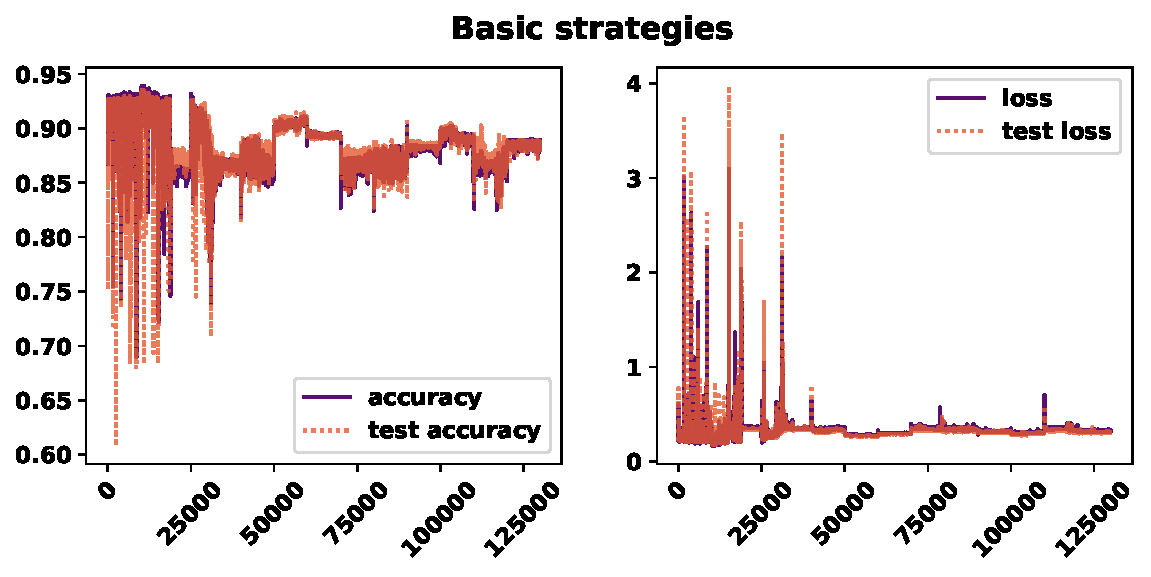
\includegraphics[width=.8\textwidth]{src/chapters/07/img/validation_plot_basic_strategies.pdf}
    \end{subfigure}
    \caption{Validation of sequence to sequence}\label{fig:validation_sequence_to_sequence}
\end{figure}

\begin{figure}[!htbp]
    \begin{subfigure}{\textwidth}
    \centering
    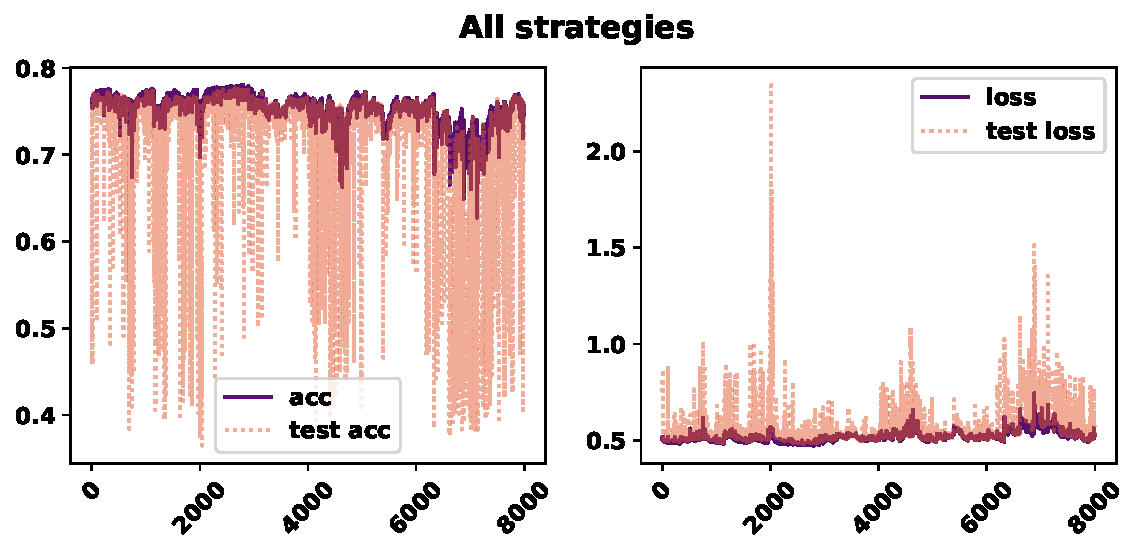
\includegraphics[width=.8\textwidth]{src/chapters/07/img/validation_plot_classification_all_strategies.pdf}
    \end{subfigure}\hfill
    \begin{subfigure}{\textwidth}
    \centering
    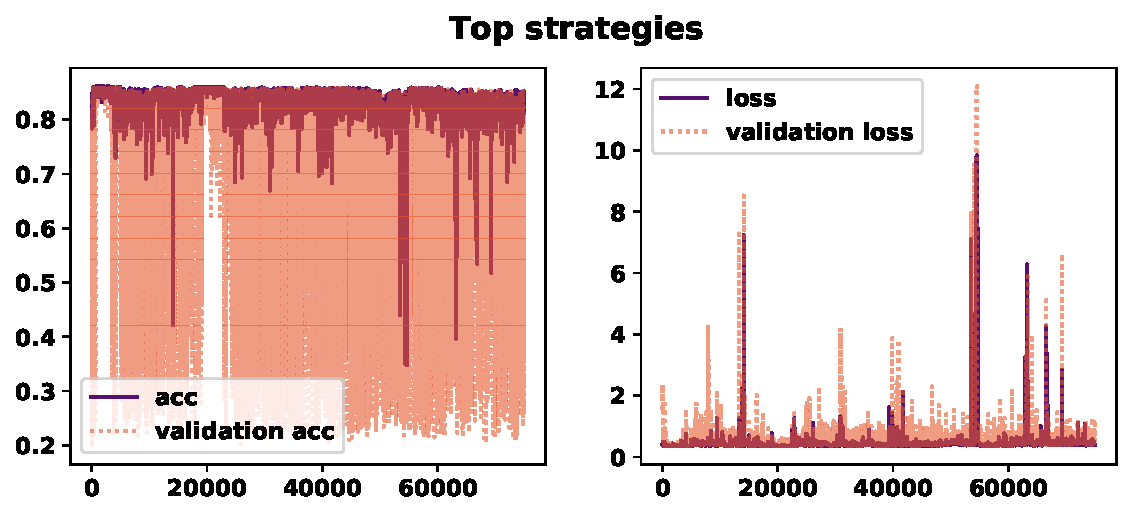
\includegraphics[width=.8\textwidth]{src/chapters/07/img/validation_plot_classification_top_strategies.pdf}
    \end{subfigure}
    \begin{subfigure}{\textwidth}
    \centering
    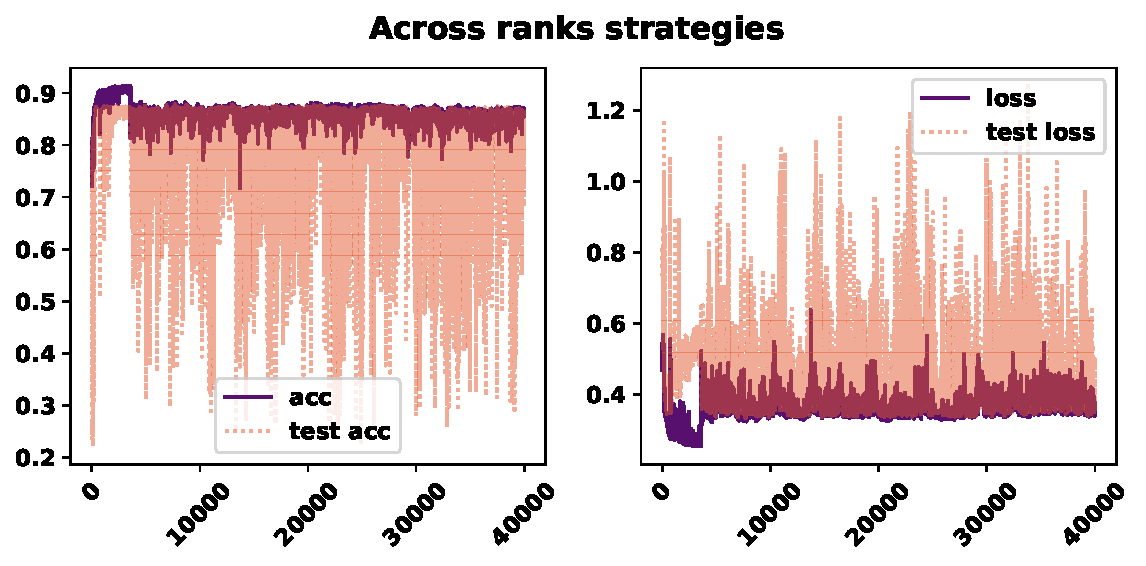
\includegraphics[width=.8\textwidth]{src/chapters/07/img/validation_plot_classification_across_ranks_strategies.pdf}
    \end{subfigure}
    \begin{subfigure}{\textwidth}
    \centering
    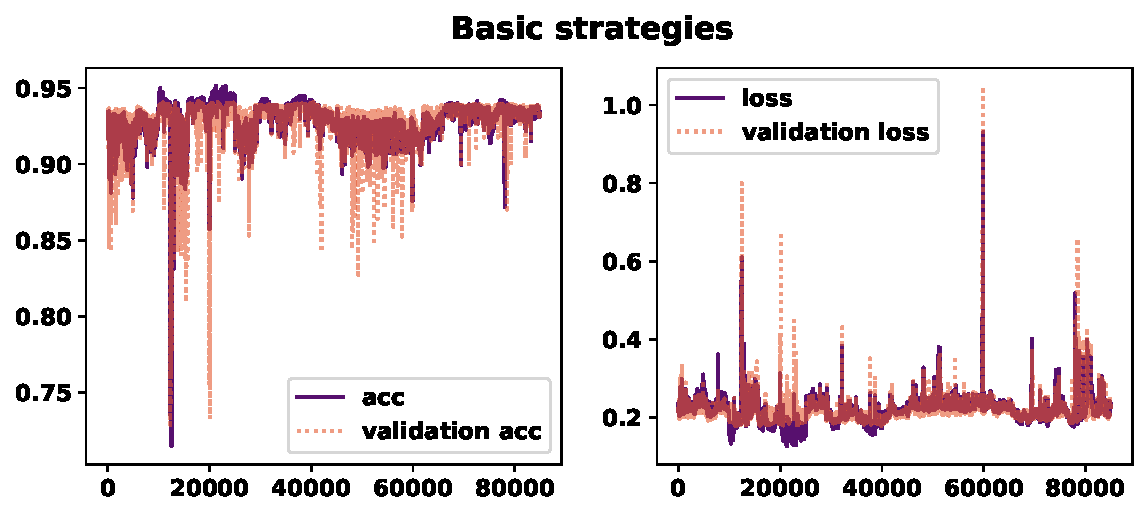
\includegraphics[width=.8\textwidth]{src/chapters/07/img/validation_plot_classification_basic_strategies.pdf}
    \end{subfigure}
    \caption{Validation of sequence to probability}\label{fig:validation_sequence_to_probability}
\end{figure}

Discussion on validation. In section~\ref{section:rnn_strategy_validation} the
LSTM networks are validated by as an IPD strategy using a meta tournament
analysis.

\section{Validation of LSTM base strategies using a meta tournament analysis}\label{section:rnn_strategy_validation}

To evaluate the LSTM players as strategies, a strategy class was implemented
that takes as an argument the a Keras model. The player then uses the history
of the match translate it to an input in the form that the networks can then
translate into an action. Note that the network was not trained to consider
it's opening move. The opening move is also an input to the strategy class.
In the meta tournament analysis different strategies that have a different
opening play are considered.

\begin{figure}[!htbp]
\begin{sourcepy}
import numpy as np

import axelrod as axl
from axelrod.random_ import random_choice
from keras.layers import LSTM, Dense, Dropout
from keras.models import Sequential

C, D = axl.Action.C, axl.Action.D


class LSTMPlayer(axl.Player):
    name = "The LSTM player"
    classifier = {
        "memory_depth": float("inf"),
        "stochastic": True,
        "inspects_source": False,
        "manipulates_source": False,
        "manipulates_state": False,
    }

    def __init__(self, model, reshape_history_funct, opening_probability=0.78):
        self.model = model
        self.opening_probability = opening_probability
        self.reshape_history_function = reshape_history_funct
        super().__init__()
        if opening_probability in [0, 1]:
            self.classifier["stochastic"] = False

    def strategy(self, opponent):
        if len(self.history) == 0:
            return random_choice(self.opening_probability)

        history = [action.value for action in opponent.history]
        prediction = float(
            self.model.predict(self.reshape_history_function(history))[0][-1]
        )

        return axl.Action(round(prediction))

    def __repr__(self):
        return self.name
\end{sourcepy}
\end{figure}

The implemented class can interact with any opponent from APL.
An example of usage of the LSTMPlayer is given by Figure.

To evaluate the performance of the LSTM strategy a meta tournament analysis,
similar to Chapter~\ref{chapter:meta_tournaments}, is carried out. The
tournament type considered here are standard tournaments. The data collections
is given by Algorithm~\ref{meta_tournament_lstm_validation}. At each trial
a number of opponents, a list of opponent From 5 to 10. The number of turns and repetitions
are fixed to 200 and 50.

The number 205 was hard coded. The evaluation does not want to take into account
the last turns. 205 was selected so the last turns could have beed discarded
and the match length would be 200 which is the number of turns commonly used
in the literature.

%TODO talk about opening probability

\begin{algorithm}[!htbp]
    \setstretch{1.35}
    \ForEach{\text{seed} $\in [0, 300]$}{
        $N \gets \text{randomly select integer}\in [N_{min}, N_{max}]$\;
        $\text{players} \gets  \text{randomly select $N$ players}$\;
        $\text{players} \gets  \text{players} + \text{LSTM strategy}$\;
        $N \gets N + 1$\;
        $k \gets  50$\;
        $n \gets  200$\;
        \vspace{0.4cm}
        $\text{result standard}$ $\gets$ Axelrod.tournament$(\text{players}, n, k)$\;}
    \KwRet{result standard}\;
    \caption{Data collection Algorithm}
    \label{algorithm:meta_tournament_lstm_validation}
\end{algorithm}

A total of \metatournamentslstm trials of
Algorithm~\ref{algorithm:meta_tournament_lstm_validation} have been performed.
Similarly to Chapter~\ref{chapter:meta_tournament} each trial outputs a result
summary of the tournament. The performance of the strategies are evaluated on
the normalised rank \(r\), and more specifically on the median normalised rank
\(\bar{r}\). A total of different strategies competed in the tournaments, and
the strategy with the maximum participation, excluding the LSTM strategy, was.

There are two distinct networks that have been trained on four different data
sets. Moreover, each networks translates into a player that the opening
probability can have three different values. Thus a total of $2 \times 4 \times
3$ LSTM players performance is evaluated in this section.

\begin{table}[!htbp]
    \begin{center}
    \resizebox{.9\textwidth}{!}{
        \begin{tabular}{lllllll}
\toprule
{} & \multicolumn{3}{c}{\textbf{sequence to sequence}} & \multicolumn{3}{c}{\textbf{sequence to probability}} \\
{} &                       $p_o=0$ &                       $p_o=1$ &                    $p_o=0.78$ &                       $p_o=0$ &                       $p_o=1$ &                    $p_o=0.78$ \\
\midrule
All strategies          &  \cellcolor{orange!67.0}0.667 &  \cellcolor{orange!22.0}0.222 &  \cellcolor{orange!33.0}0.333 &  \cellcolor{orange!78.0}0.778 &  \cellcolor{orange!33.0}0.333 &    \cellcolor{orange!50.0}0.500 \\
Top strategies          &  \cellcolor{orange!71.0}0.714 &  \cellcolor{orange!44.0}0.444 &    \cellcolor{orange!50.0}0.500 &    \cellcolor{orange!50.0}0.500 &  \cellcolor{orange!43.0}0.429 &  \cellcolor{orange!43.0}0.429 \\
Across ranks strategies &   \cellcolor{orange!75.0}0.750 &  \cellcolor{orange!67.0}0.667 &  \cellcolor{orange!68.0}0.683 &    \cellcolor{orange!50.0}0.500 &   \cellcolor{orange!25.0}0.250 &    \cellcolor{orange!30.0}0.300 \\
Basic strategies        &    \cellcolor{orange!80.0}0.800 &    \cellcolor{orange!60.0}0.600 &  \cellcolor{orange!62.0}0.625 &    \cellcolor{orange!80.0}0.800 &    \cellcolor{orange!30.0}0.300 &  \cellcolor{orange!43.0}0.429 \\
\bottomrule
\end{tabular}

    }
\end{center}
\caption{Median normalised ranks of th 24 LSTM strategies over standard tournaments.}
% \label{table:normalised_rank_lstm_tournaments}
\end{table}

\begin{figure}[!htbp]
    \begin{subfigure}{\textwidth}
    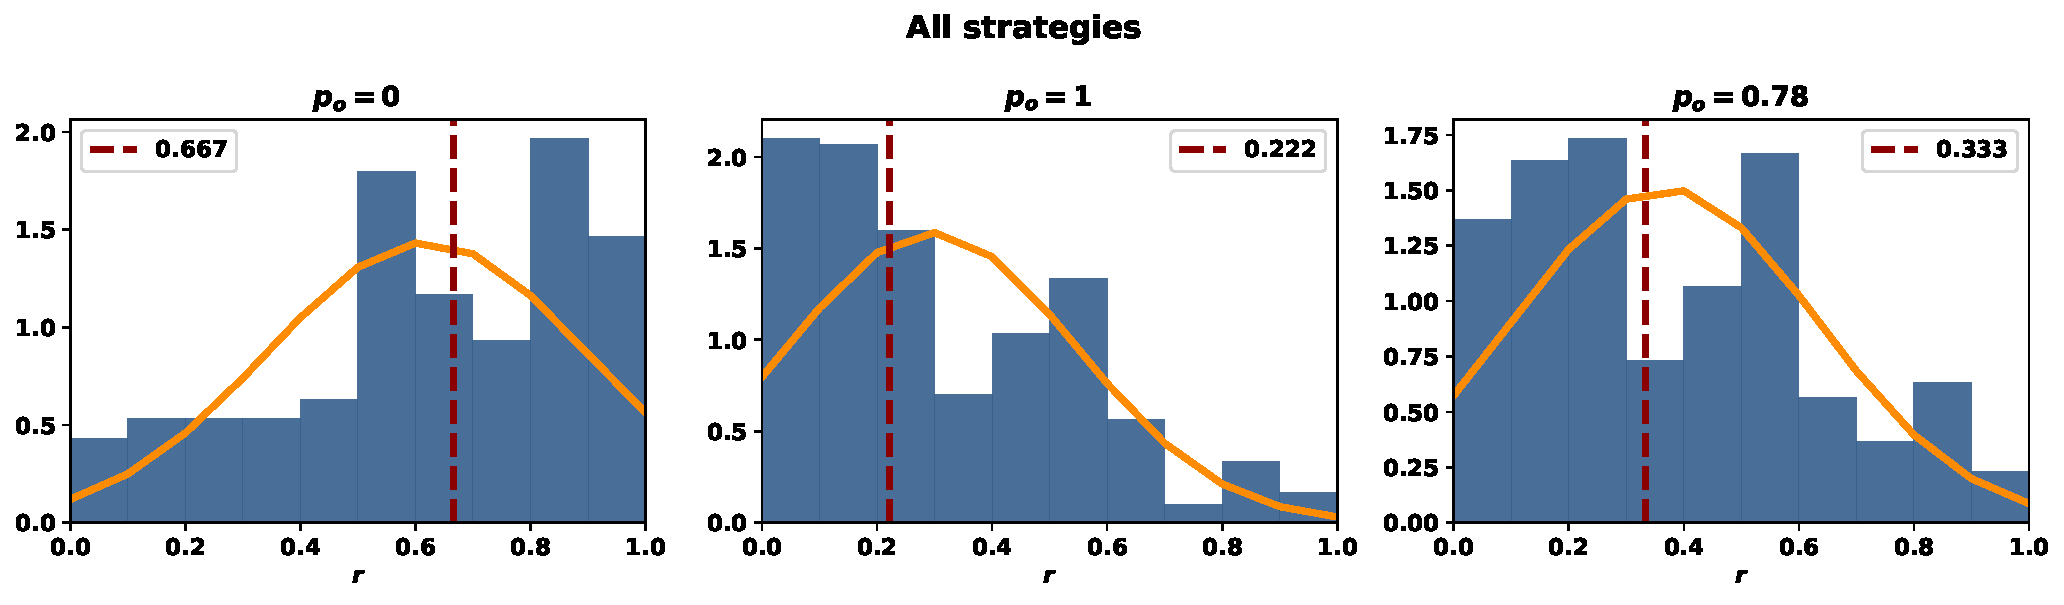
\includegraphics[width=\textwidth]{src/chapters/07/img/normalised_rank_all_strategies.pdf}
    \end{subfigure}
    \par\bigskip
    \begin{subfigure}{\textwidth}
    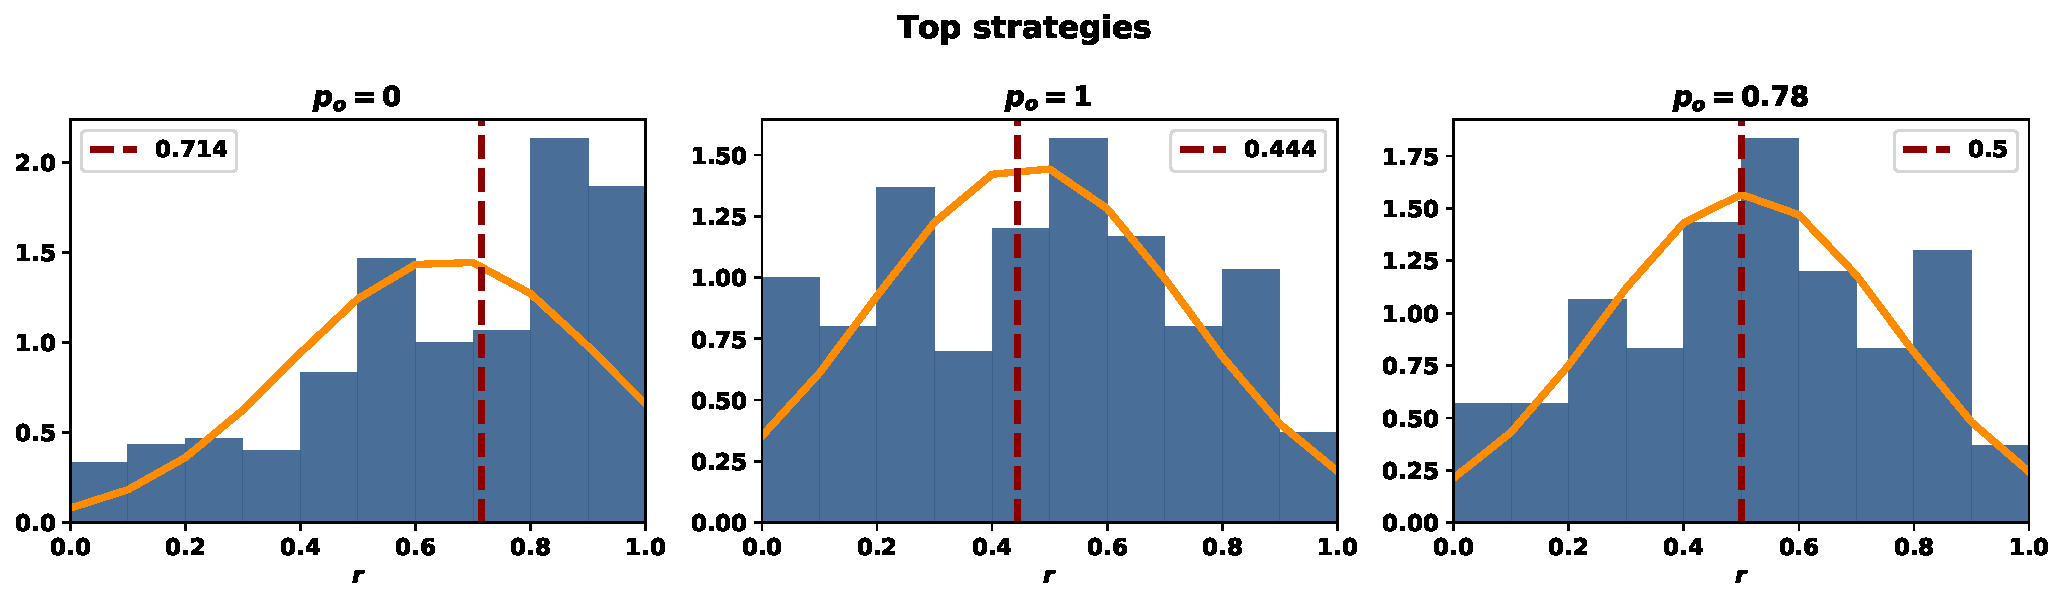
\includegraphics[width=\textwidth]{src/chapters/07/img/normalised_rank_top_strategies.pdf}
    \end{subfigure}
    \par\bigskip
    \begin{subfigure}{\textwidth}
    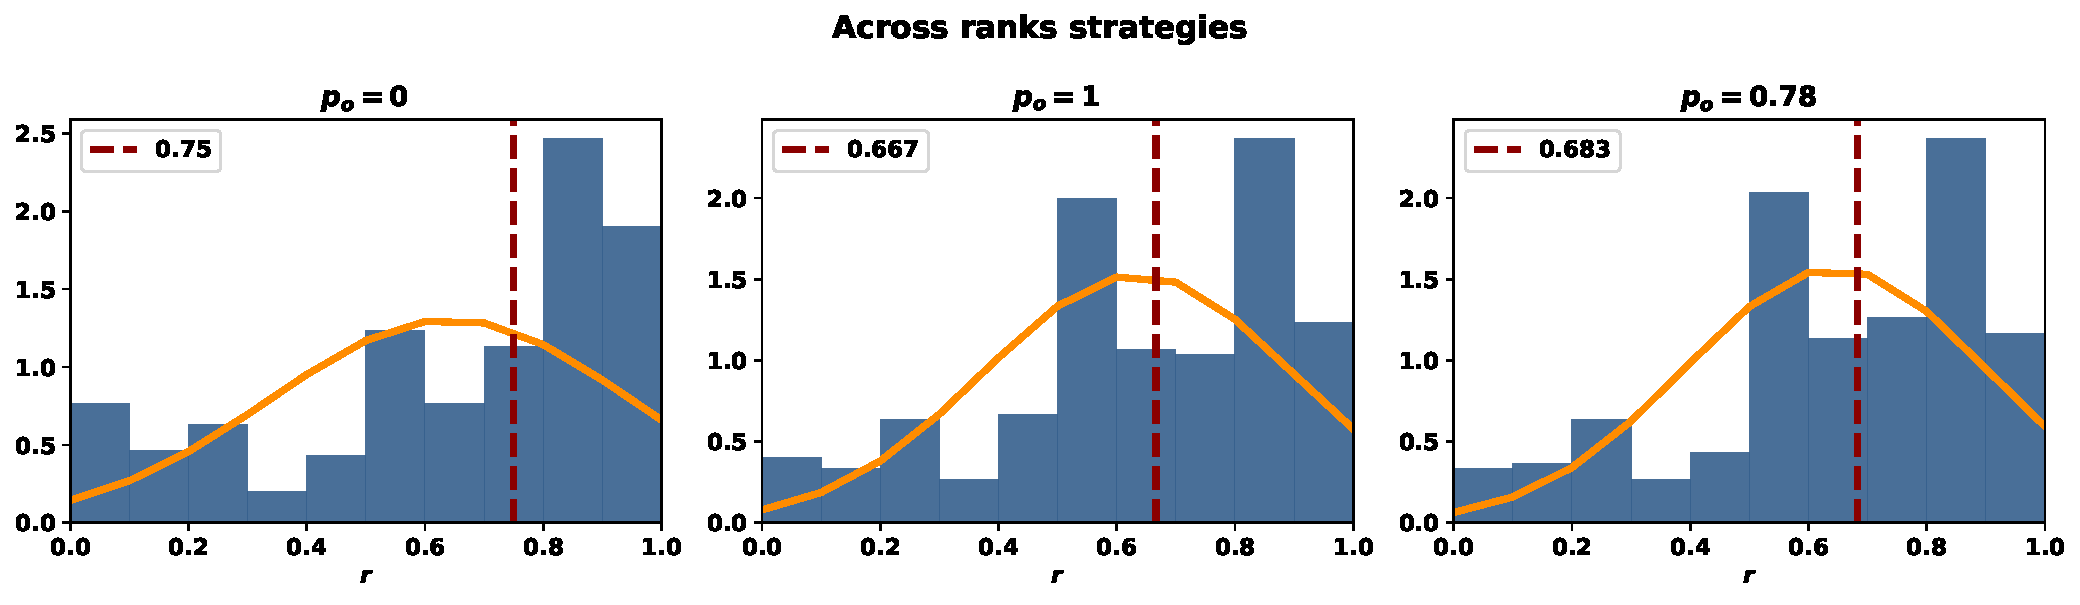
\includegraphics[width=\textwidth]{src/chapters/07/img/normalised_rank_across_ranks_strategies.pdf}
    \end{subfigure}
    \par\bigskip
    \begin{subfigure}{\textwidth}
    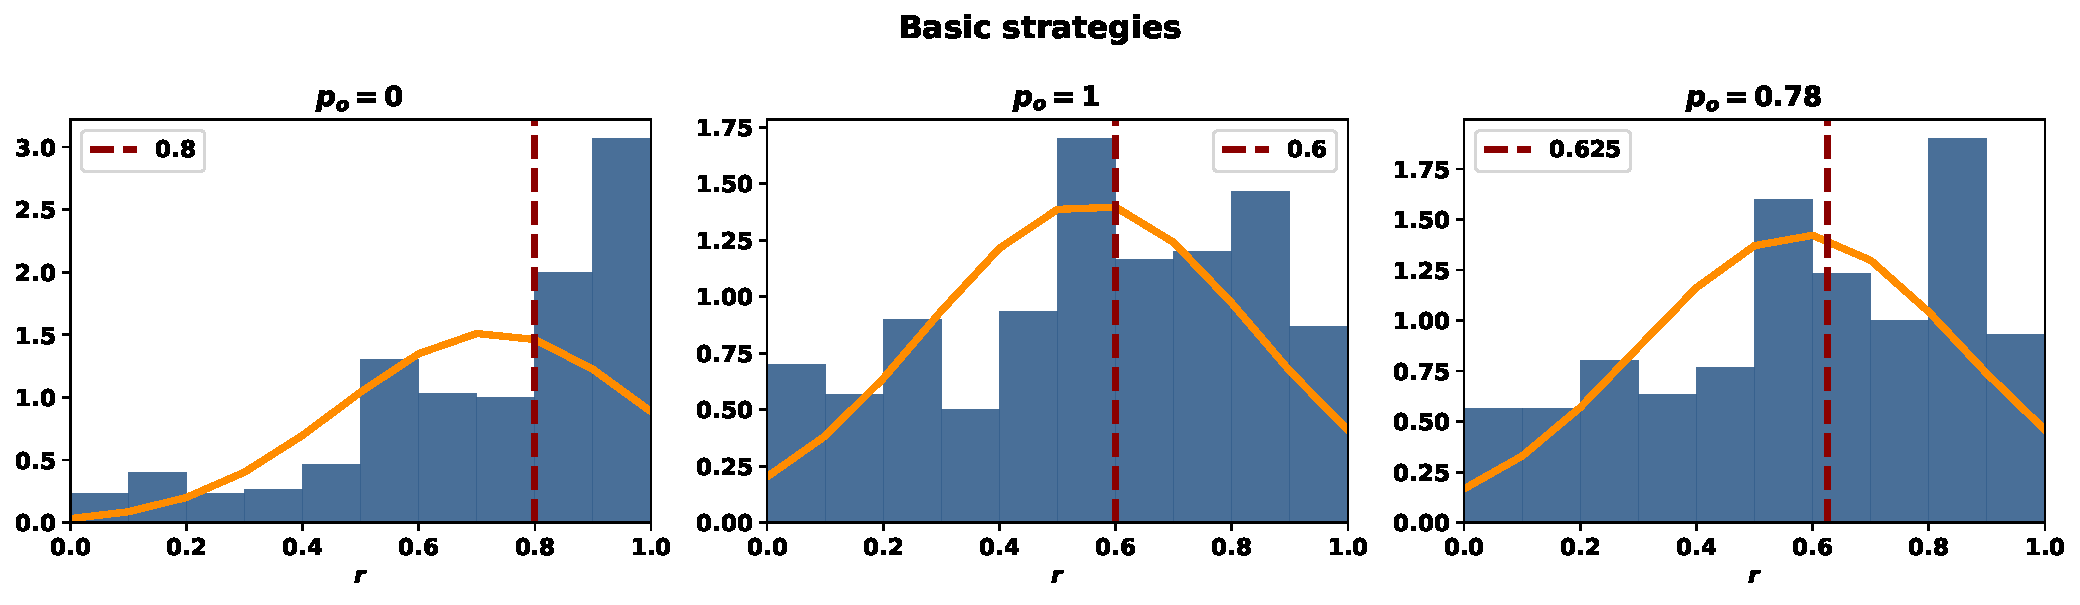
\includegraphics[width=\textwidth]{src/chapters/07/img/normalised_rank_basic_strategies.pdf}
    \end{subfigure}
    % \caption{Validation of sequence to sequence}\label{fig:validation_sequence_to_sequence}
\end{figure}


\begin{table}[!htbp]
    \begin{center}
    \resizebox{.9\textwidth}{!}{
        \begin{tabular}{llrrrrrrrrrrrr}
\toprule
                 &            &  count &   mean &    std &  min &    10\% &    25\% &    50\% &    75\% &    95\% &  max &   skew &   kurt \\
\midrule
\rowcolor{Gray}
All strategies & $p_o=0$ &  300.0 &  0.620 &  0.278 &  0.0 &  0.200 &  0.429 &  0.667 &  0.839 &  1.000 &  1.0 & -0.523 & -0.587 \\
\rowcolor{Gray}
                 & $p_o=1$ &  300.0 &  0.295 &  0.252 &  0.0 &  0.000 &  0.111 &  0.222 &  0.458 &  0.779 &  1.0 &  0.702 & -0.251 \\
\rowcolor{Gray}
                 & $p_o=0.78$ &  300.0 &  0.368 &  0.265 &  0.0 &  0.000 &  0.143 &  0.333 &  0.560 &  0.833 &  1.0 &  0.433 & -0.647 \\
                 \midrule
Top strategies & $p_o=0$ &  300.0 &  0.655 &  0.273 &  0.0 &  0.250 &  0.500 &  0.714 &  0.875 &  1.000 &  1.0 & -0.629 & -0.436 \\
                 & $p_o=1$ &  300.0 &  0.461 &  0.274 &  0.0 &  0.090 &  0.222 &  0.444 &  0.667 &  0.875 &  1.0 & -0.029 & -0.940 \\
                 & $p_o=0.78$ &  300.0 &  0.509 &  0.255 &  0.0 &  0.167 &  0.333 &  0.500 &  0.704 &  0.876 &  1.0 & -0.158 & -0.710 \\
                 \midrule
\rowcolor{Gray}
Representative strategies & $p_o=0$ &  300.0 &  0.643 &  0.306 &  0.0 &  0.141 &  0.486 &  0.750 &  0.875 &  1.000 &  1.0 & -0.768 & -0.523 \\
\rowcolor{Gray}
                 & $p_o=1$ &  300.0 &  0.636 &  0.262 &  0.0 &  0.250 &  0.500 &  0.667 &  0.833 &  1.000 &  1.0 & -0.680 & -0.198 \\
\rowcolor{Gray}
                 & $p_o=0.78$ &  300.0 &  0.645 &  0.255 &  0.0 &  0.250 &  0.500 &  0.683 &  0.833 &  1.000 &  1.0 & -0.754 & -0.034 \\
                 \midrule
Basic strategies & $p_o=0$ &  300.0 &  0.728 &  0.263 &  0.0 &  0.333 &  0.600 &  0.800 &  1.000 &  1.000 &  1.0 & -0.949 &  0.229 \\
                 & $p_o=1$ &  300.0 &  0.556 &  0.283 &  0.0 &  0.143 &  0.375 &  0.600 &  0.778 &  1.000 &  1.0 & -0.365 & -0.803 \\
                 & $p_o=0.78$ &  300.0 &  0.579 &  0.280 &  0.0 &  0.167 &  0.375 &  0.625 &  0.800 &  1.000 &  1.0 & -0.435 & -0.772 \\
\bottomrule
\end{tabular}

    }
\end{center}
% \caption{Number of epochs each both networks, sequence to sequence and 
% sequence to probability, were trained for each subset.}\label{table:epochs}
\end{table}


\begin{figure}[!htbp]
    \begin{subfigure}{\textwidth}
    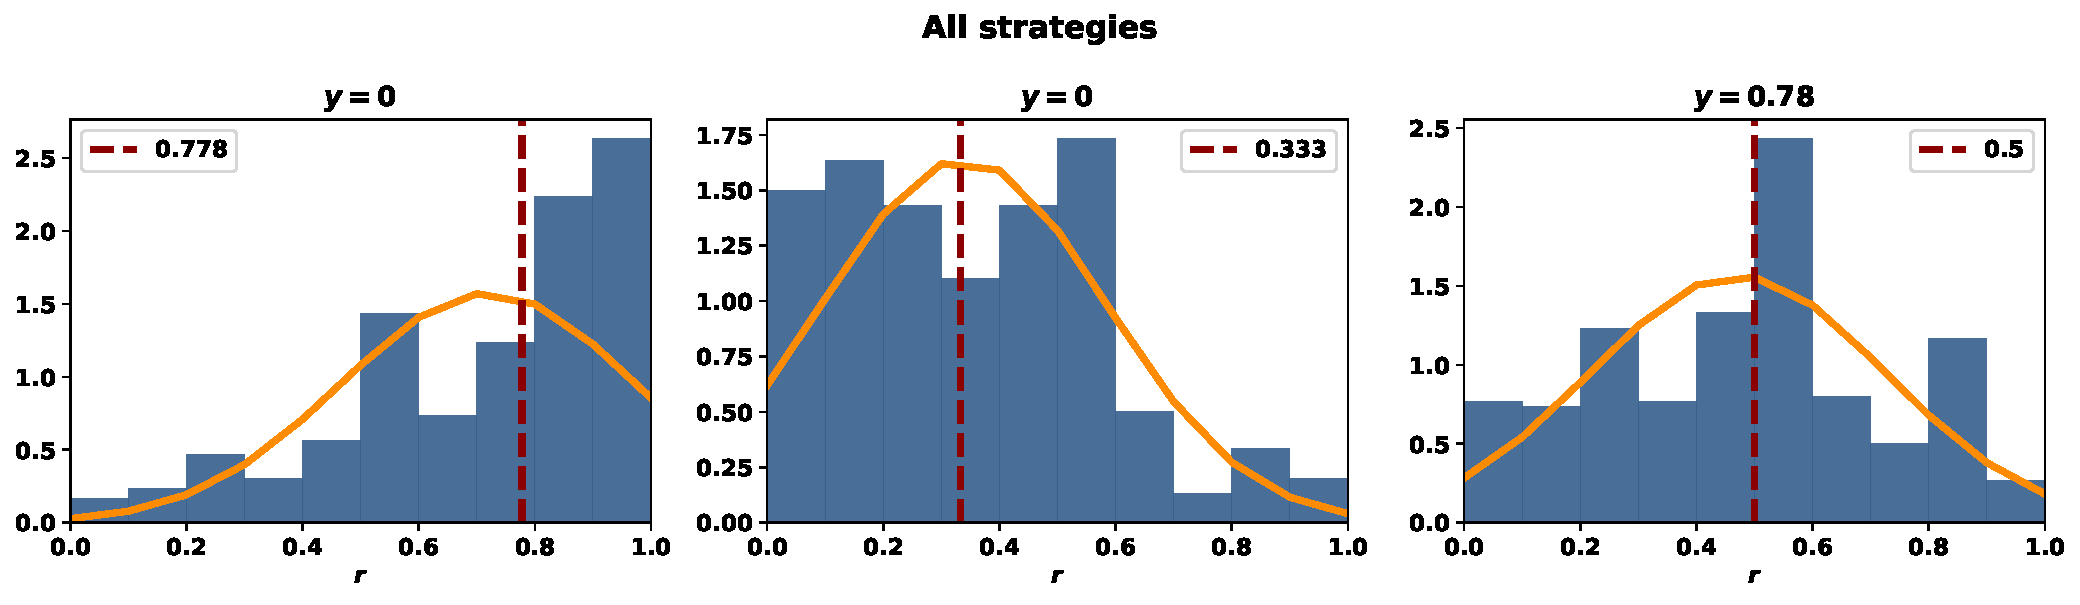
\includegraphics[width=\textwidth]{src/chapters/07/img/normalised_rank_classification_all_strategies.pdf}
    \end{subfigure}
    \par\bigskip
    \begin{subfigure}{\textwidth}
    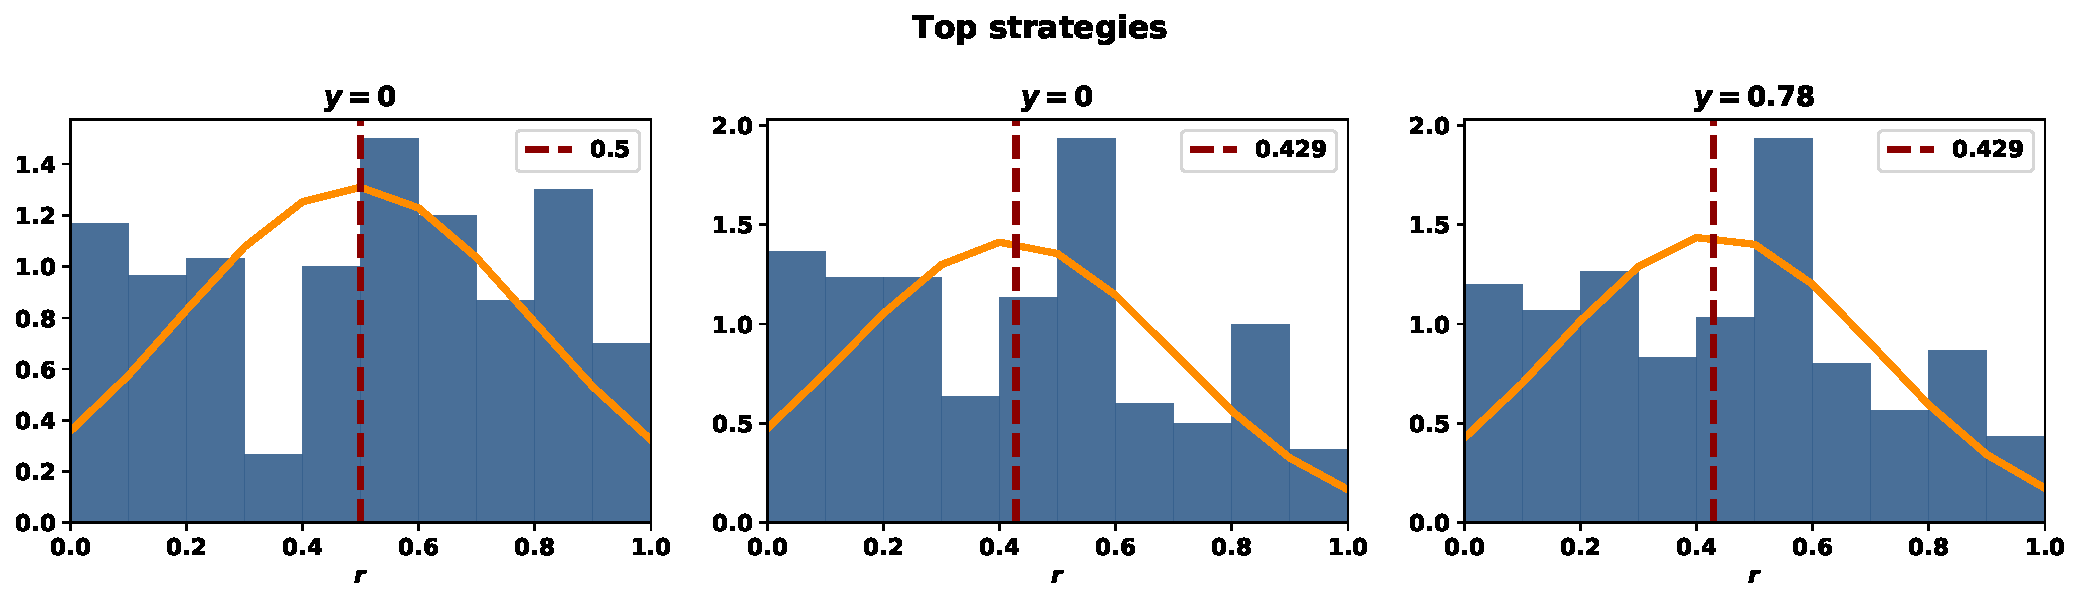
\includegraphics[width=\textwidth]{src/chapters/07/img/normalised_rank_classification_top_strategies.pdf}
    \end{subfigure}
    \par\bigskip
    \begin{subfigure}{\textwidth}
    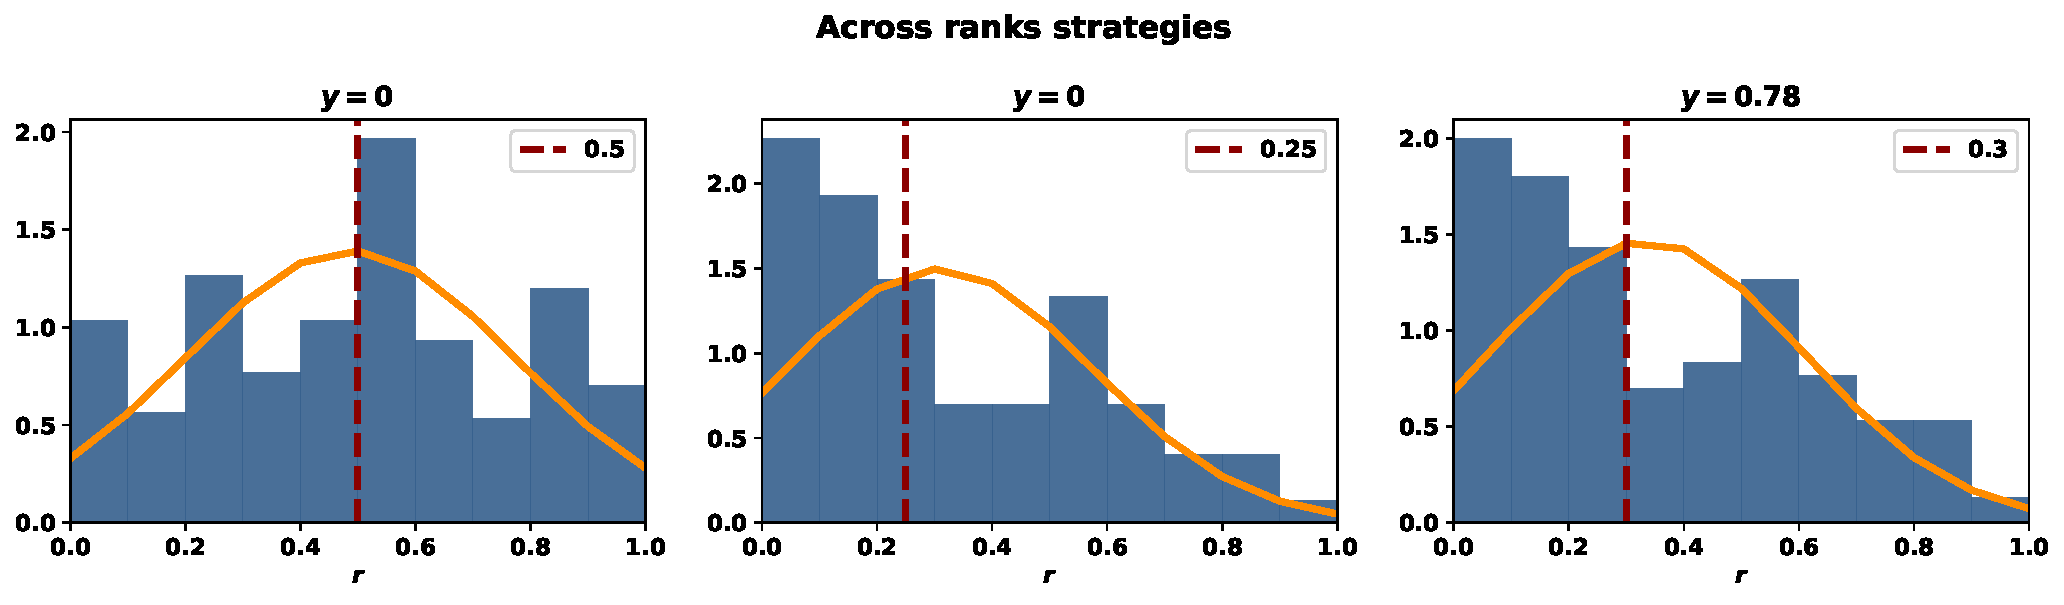
\includegraphics[width=\textwidth]{src/chapters/07/img/normalised_rank_classification_across_ranks_strategies.pdf}
    \end{subfigure}
    \par\bigskip
    \begin{subfigure}{\textwidth}
    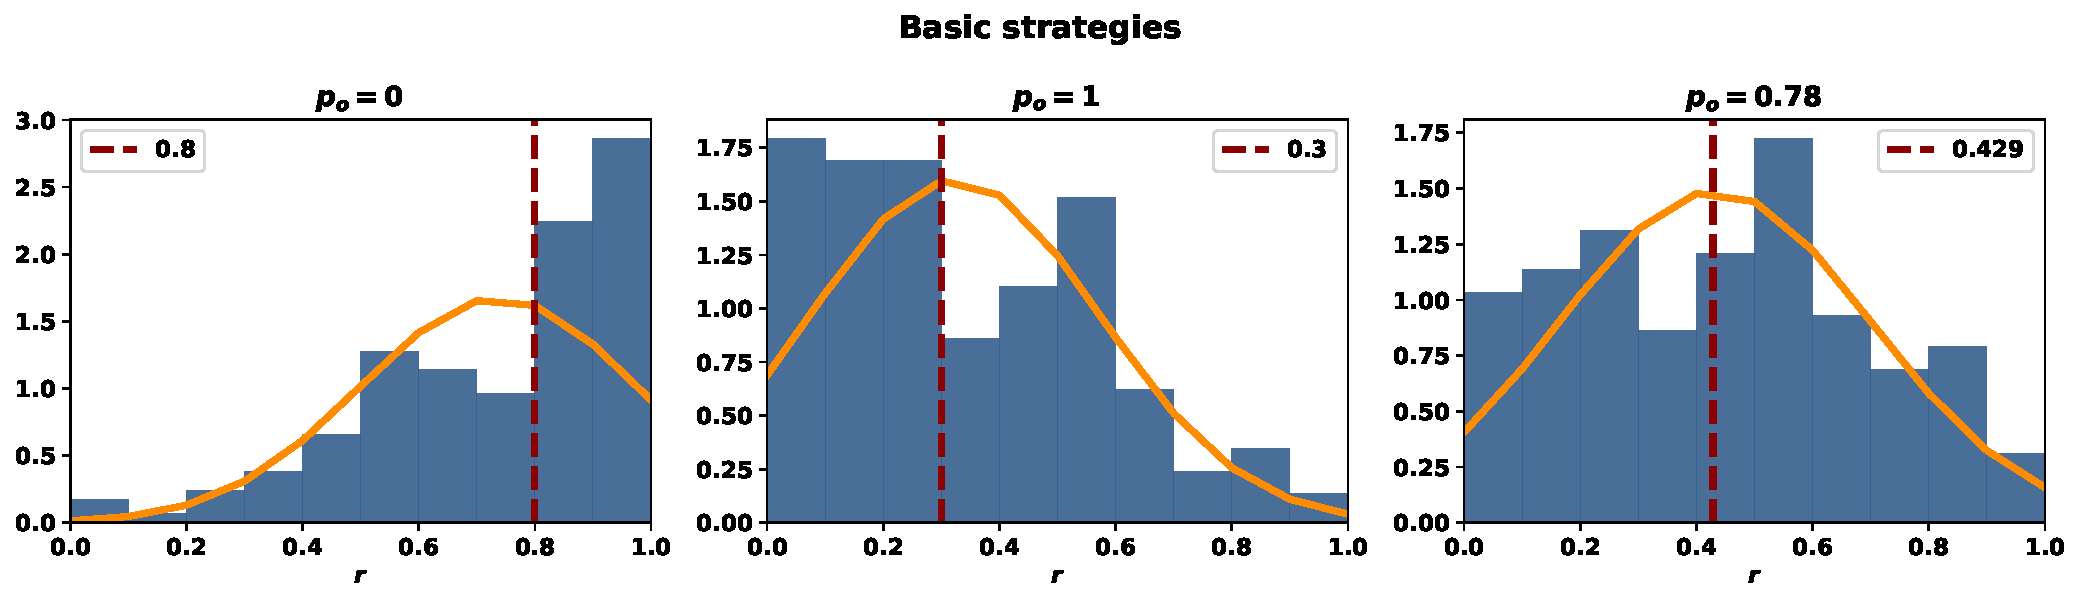
\includegraphics[width=\textwidth]{src/chapters/07/img/normalised_rank_classification_basic_strategies.pdf}
    \end{subfigure}
    % \caption{Validation of sequence to probability}\label{fig:validation_sequence_to_probability}
\end{figure}

\begin{table}[!htbp]
    \begin{center}
    \resizebox{.9\textwidth}{!}{
        \begin{tabular}{llrrrrrrrrrrrr}
\toprule
                 &            &  count &   mean &    std &  min &    10\% &    25\% &    50\% &    75\% &    95\% &  max &   skew &   kurt \\
\midrule
\rowcolor{Gray}
All strategies & $p_o=0$ &  300.0 &  0.720 &  0.254 &  0.0 &  0.333 &  0.571 &  0.778 &  0.900 &  1.000 &  1.0 & -0.860 &  0.056 \\
\rowcolor{Gray}
                 & $p_o=1$ &  300.0 &  0.339 &  0.244 &  0.0 &  0.000 &  0.125 &  0.333 &  0.500 &  0.800 &  1.0 &  0.458 & -0.280 \\
\rowcolor{Gray}
                 & $p_o=0.78$ &  300.0 &  0.471 &  0.255 &  0.0 &  0.125 &  0.286 &  0.500 &  0.625 &  0.875 &  1.0 & -0.064 & -0.696 \\
                 \midrule
Top strategies & $p_o=0$ &  300.0 &  0.491 &  0.305 &  0.0 &  0.000 &  0.200 &  0.500 &  0.714 &  1.000 &  1.0 & -0.131 & -1.140 \\
                 & $p_o=1$ &  300.0 &  0.417 &  0.283 &  0.0 &  0.000 &  0.167 &  0.429 &  0.600 &  0.875 &  1.0 &  0.157 & -0.974 \\
                 & $p_o=0.78$ &  300.0 &  0.432 &  0.277 &  0.0 &  0.000 &  0.200 &  0.429 &  0.625 &  0.876 &  1.0 &  0.109 & -0.891 \\
                 \midrule
\rowcolor{Gray}
Across ranks strategies & $p_o=0$ &  300.0 &  0.487 &  0.287 &  0.0 &  0.000 &  0.286 &  0.500 &  0.700 &  1.000 &  1.0 & -0.037 & -0.899 \\
\rowcolor{Gray}
                 & $p_o=1$ &  300.0 &  0.308 &  0.267 &  0.0 &  0.000 &  0.111 &  0.250 &  0.500 &  0.800 &  1.0 &  0.586 & -0.695 \\
\rowcolor{Gray}
                 & $p_o=0.78$ &  300.0 &  0.335 &  0.272 &  0.0 &  0.000 &  0.125 &  0.300 &  0.556 &  0.800 &  1.0 &  0.465 & -0.867 \\
                 \midrule
Basic strategies & $p_o=0$ &  290.0 &  0.738 &  0.239 &  0.0 &  0.400 &  0.600 &  0.800 &  0.975 &  1.000 &  1.0 & -0.881 &  0.315 \\
                 & $p_o=1$ &  290.0 &  0.323 &  0.249 &  0.0 &  0.000 &  0.125 &  0.300 &  0.500 &  0.778 &  1.0 &  0.491 & -0.535 \\
                 & $p_o=0.78$ &  290.0 &  0.432 &  0.269 &  0.0 &  0.000 &  0.200 &  0.429 &  0.625 &  0.875 &  1.0 &  0.096 & -0.916 \\
\bottomrule
\end{tabular}

    }
\end{center}
% \caption{Number of epochs each both networks, sequence to sequence and 
% sequence to probability, were trained for each subset.}\label{table:epochs}
\end{table}

\begin{figure}[!htbp]
    \begin{subfigure}{.45\textwidth}
    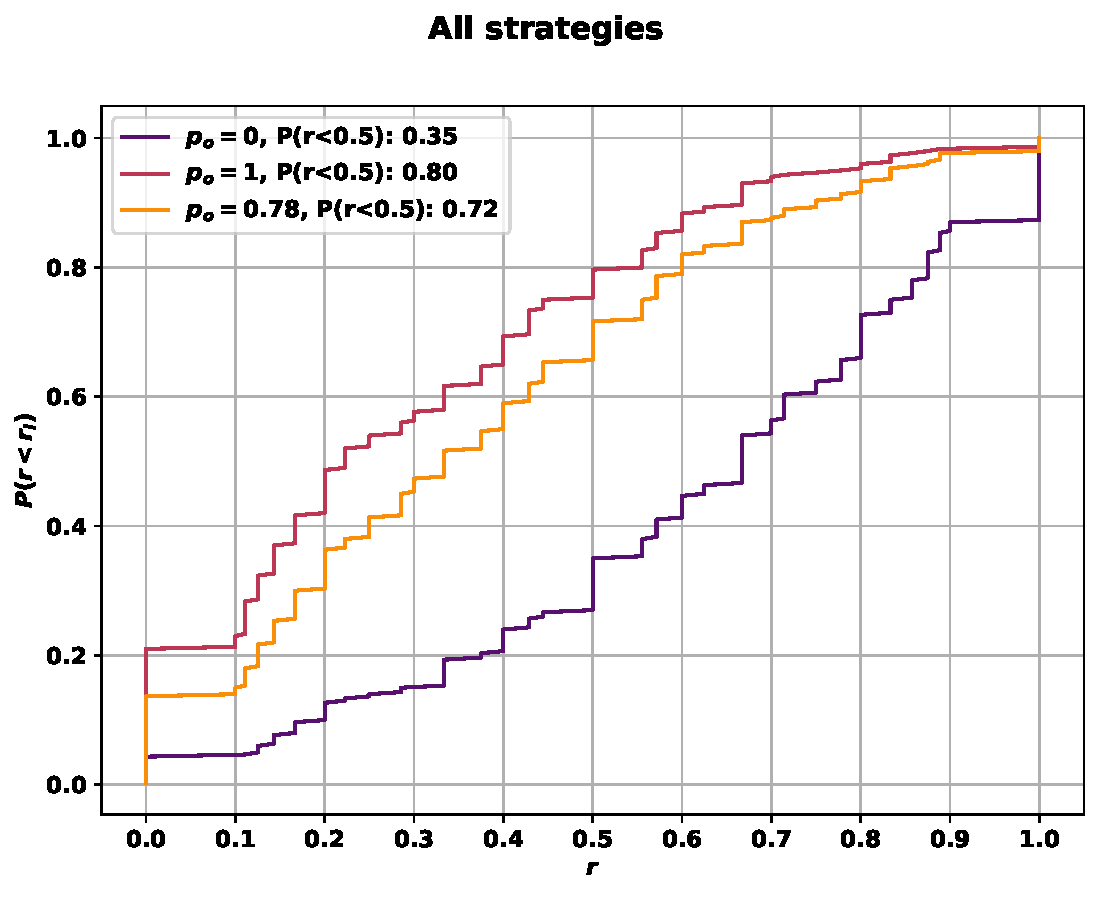
\includegraphics[width=\textwidth]{src/chapters/07/img/cfd_to_sequence_all_strategies.pdf}
    \caption{\(P(r<0.5): 0.350 P(r<0.5): 0.797 P(r<0.5): 0.717\)}
    \end{subfigure}\hfill
    \begin{subfigure}{.45\textwidth}
    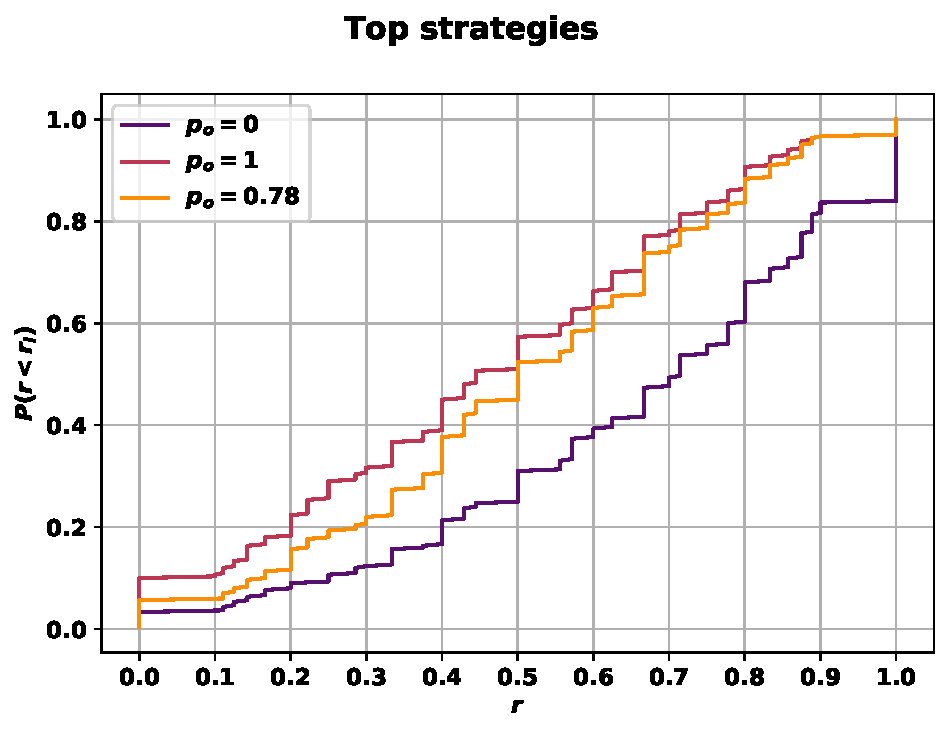
\includegraphics[width=\textwidth]{src/chapters/07/img/cfd_to_sequence_top_strategies.pdf}
    \caption{\(P(r<0.5): 0.310 P(r<0.5): 0.573 P(r<0.5): 0.523\)}
    \end{subfigure}
    \begin{subfigure}{.45\textwidth}
    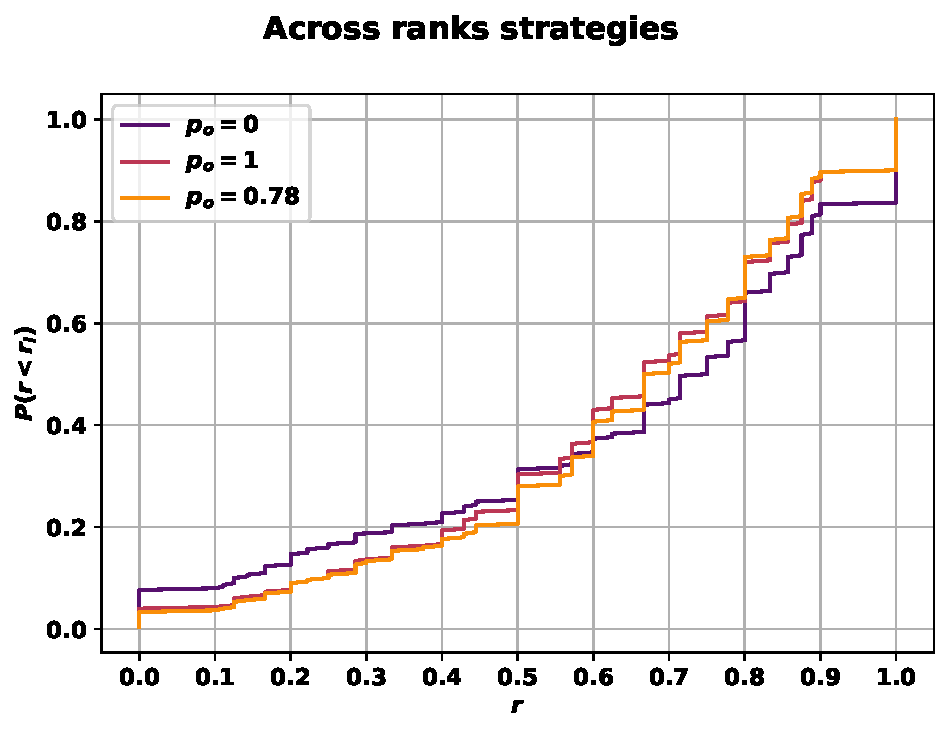
\includegraphics[width=\textwidth]{src/chapters/07/img/cfd_to_sequence_across_ranks_strategies.pdf}
    \caption(\(P(r<0.5): 0.313 P(r<0.5): 0.303 P(r<0.5): 0.280\))
    \end{subfigure}\hfill
    \begin{subfigure}{.45\textwidth}
    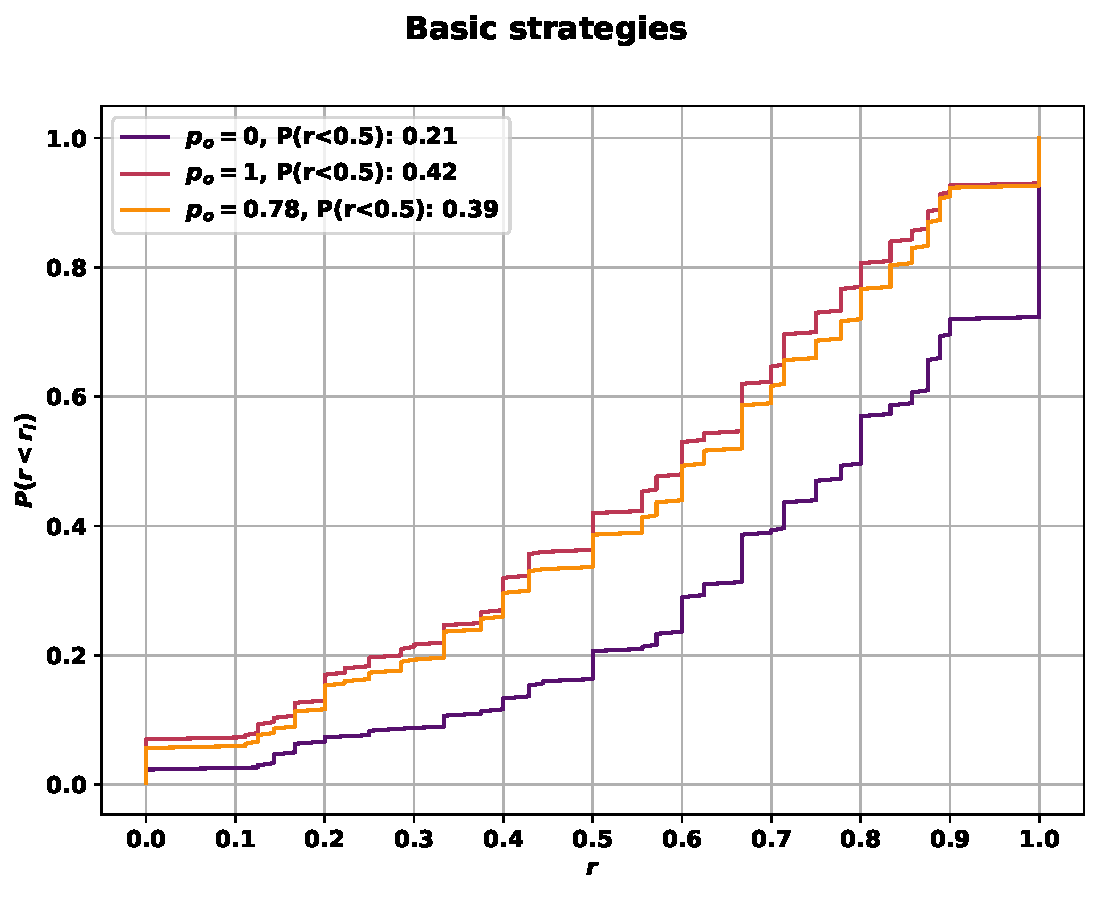
\includegraphics[width=\textwidth]{src/chapters/07/img/cfd_to_sequence_basic_strategies.pdf}
    \caption{\(P(r<0.5): 0.207 P(r<0.5): 0.420 P(r<0.5): 0.387\)}
    \end{subfigure}
    % \caption{Validation of sequence to probability}\label{fig:validation_sequence_to_probability}
\end{figure}


\begin{figure}[!htbp]
    \begin{subfigure}{.45\textwidth}
    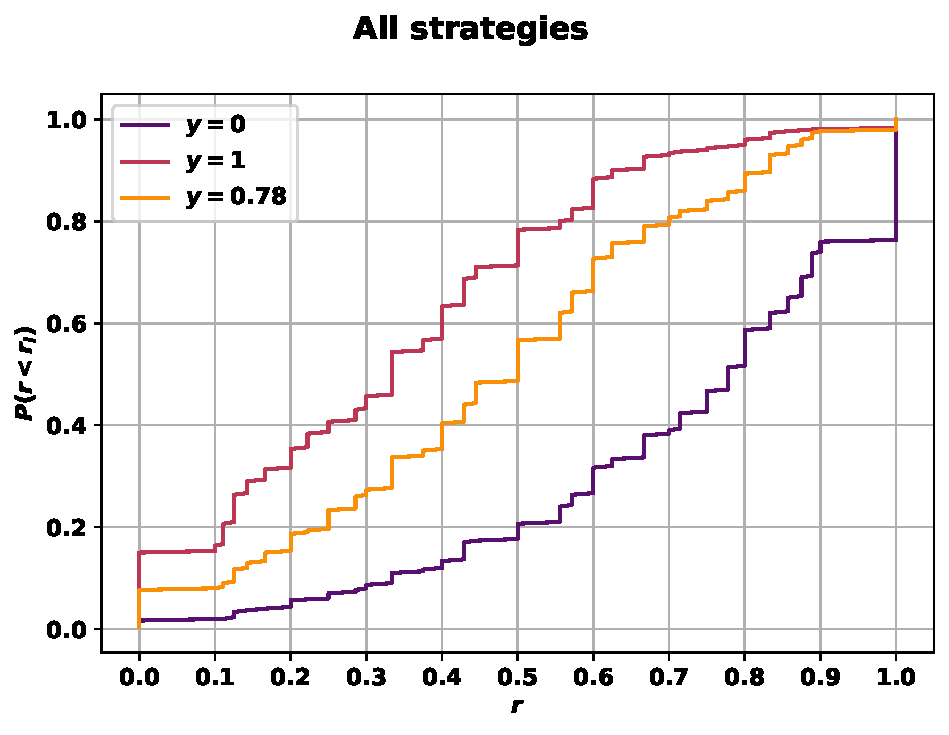
\includegraphics[width=\textwidth]{src/chapters/07/img/cfd_to_probability_all_strategies.pdf}
    \caption{\(P(r<0.5): 0.207 P(r<0.5): 0.783 P(r<0.5): 0.567\)}
    \end{subfigure}\hfill
    \begin{subfigure}{.45\textwidth}
    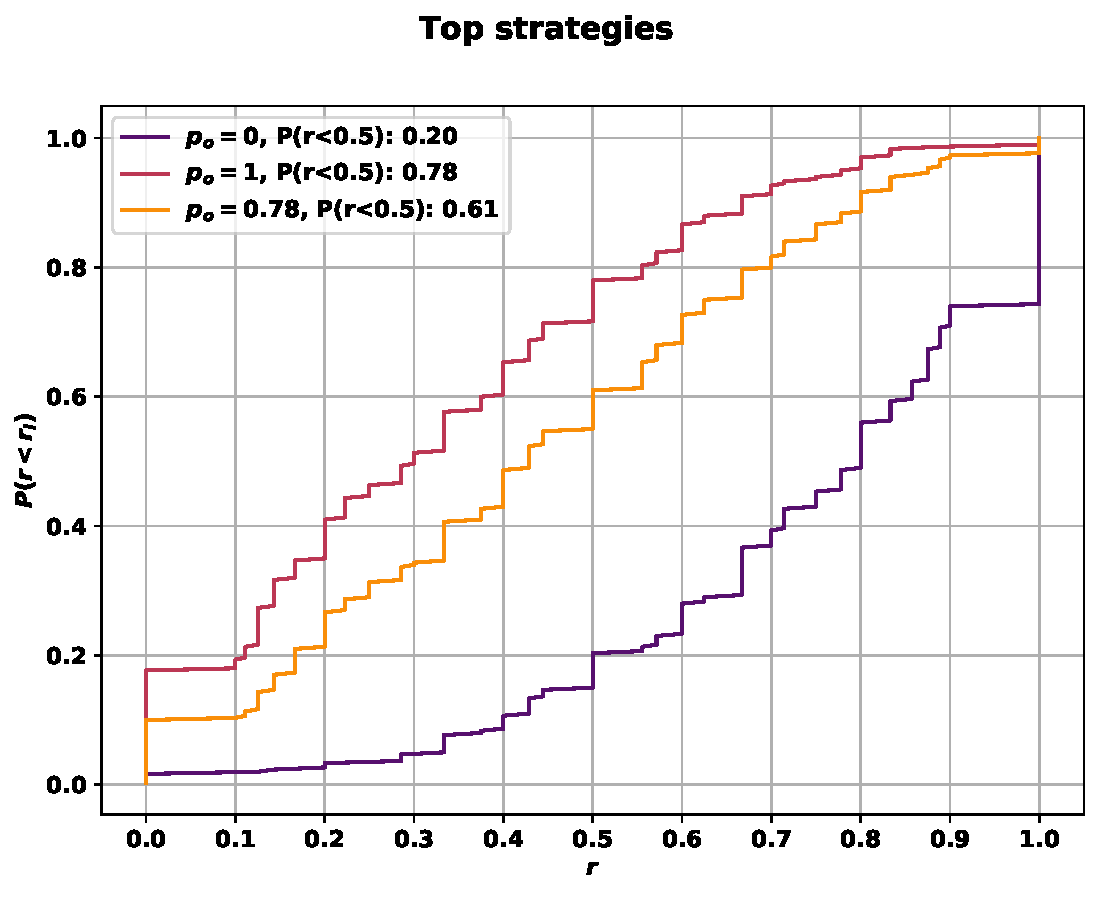
\includegraphics[width=\textwidth]{src/chapters/07/img/cfd_to_probability_top_strategies.pdf}
    \caption{\(P(r<0.5): 0.503 P(r<0.5): 0.633 P(r<0.5): 0.610\)}
    \end{subfigure}
    \begin{subfigure}{.45\textwidth}
    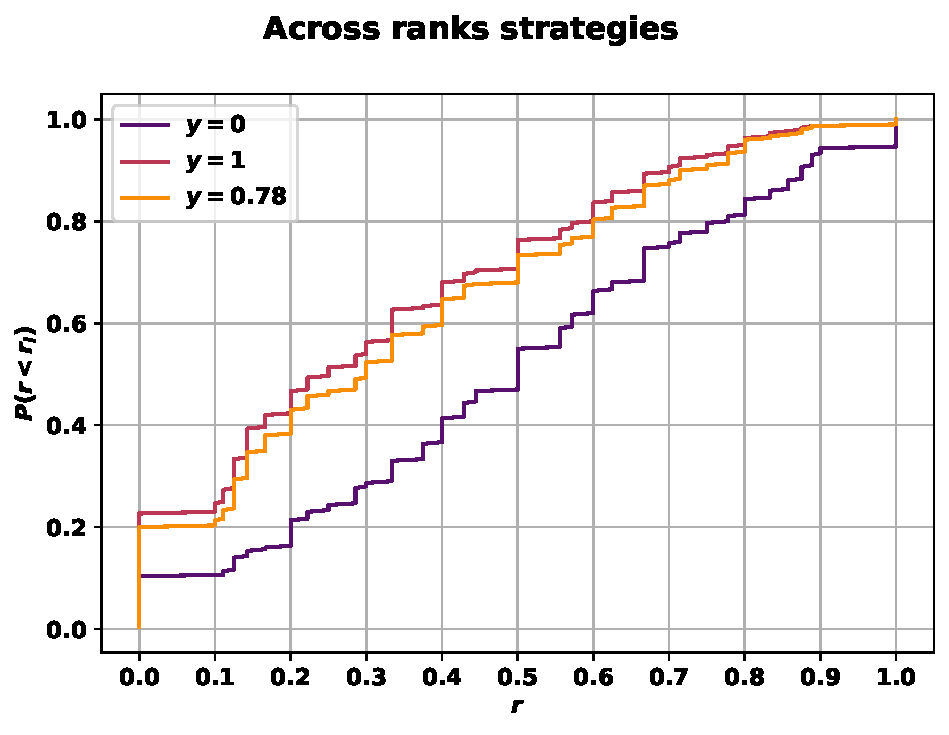
\includegraphics[width=\textwidth]{src/chapters/07/img/cfd_to_probability_across_ranks_strategies.pdf}
    \caption(\(P(r<0.5): 0.550 P(r<0.5): 0.763 P(r<0.5): 0.733\))
    \end{subfigure}\hfill
    \begin{subfigure}{.45\textwidth}
    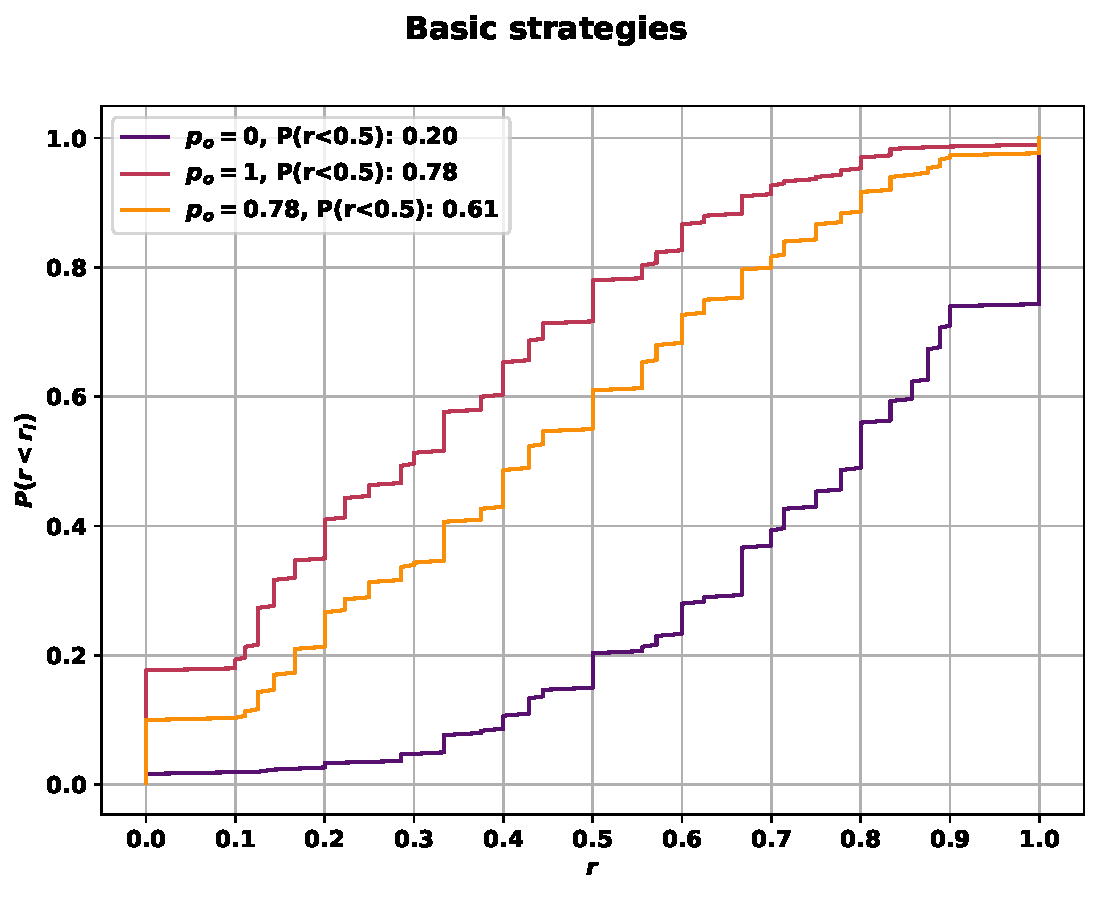
\includegraphics[width=\textwidth]{src/chapters/07/img/cfd_to_probability_basic_strategies.pdf}
    \caption{\(P(r<0.5): 0.207, P(r<0.5): 0.779, P(r<0.5): 0.607\)}
    \end{subfigure}
    % \caption{Validation of sequence to probability}\label{fig:validation_sequence_to_probability}
\end{figure}

\subsection{Fingerprinting the LSTM based strategies}

\newpage

\begin{figure}[!htbp]
    \begin{subfigure}{\textwidth}
        \includegraphics[width=.3\textwidth]{"src/chapters/07/img/Tit For Tat_lstm_sequence_0".pdf}
        \includegraphics[width=.3\textwidth]{"src/chapters/07/img/Tit For Tat_lstm_sequence_1".pdf}
        \includegraphics[width=.3\textwidth]{"src/chapters/07/img/Tit For Tat_lstm_sequence_0_78".pdf}
    \end{subfigure}
    \begin{subfigure}{\textwidth}
        \includegraphics[width=.3\textwidth]{"src/chapters/07/img/Tit For Tat_top_twenty_sequence_0".pdf}
        \includegraphics[width=.3\textwidth]{"src/chapters/07/img/Tit For Tat_top_twenty_sequence_1".pdf}
        \includegraphics[width=.3\textwidth]{"src/chapters/07/img/Tit For Tat_top_twenty_sequence_0_78".pdf}
    \end{subfigure}
    \begin{subfigure}{\textwidth}
        \includegraphics[width=.3\textwidth]{"src/chapters/07/img/Tit For Tat_twenty_sequence_0".pdf}
        \includegraphics[width=.3\textwidth]{"src/chapters/07/img/Tit For Tat_twenty_sequence_1".pdf}
        \includegraphics[width=.3\textwidth]{"src/chapters/07/img/Tit For Tat_twenty_sequence_0_78".pdf}
    \end{subfigure}
    \begin{subfigure}{\textwidth}
        \includegraphics[width=.3\textwidth]{"src/chapters/07/img/Tit For Tat_basic_sequence_0".pdf}
        \includegraphics[width=.3\textwidth]{"src/chapters/07/img/Tit For Tat_basic_sequence_1".pdf}
        \includegraphics[width=.3\textwidth]{"src/chapters/07/img/Tit For Tat_basic_sequence_0_78".pdf}
    \end{subfigure}
\end{figure}

\begin{figure}[!htbp]
    \begin{subfigure}{\textwidth}
        \includegraphics[width=.3\textwidth]{"src/chapters/07/img/Tit For Tat_lstm_classification_0".pdf}
        \includegraphics[width=.3\textwidth]{"src/chapters/07/img/Tit For Tat_lstm_classification_1".pdf}
        \includegraphics[width=.3\textwidth]{"src/chapters/07/img/Tit For Tat_lstm_classification_0_78".pdf}
    \end{subfigure}
    \begin{subfigure}{\textwidth}
        \includegraphics[width=.3\textwidth]{"src/chapters/07/img/Tit For Tat_top_twenty_classification_0".pdf}
        \includegraphics[width=.3\textwidth]{"src/chapters/07/img/Tit For Tat_top_twenty_classification_1".pdf}
        \includegraphics[width=.3\textwidth]{"src/chapters/07/img/Tit For Tat_top_twenty_classification_0_78".pdf}
    \end{subfigure}
    \begin{subfigure}{\textwidth}
        \includegraphics[width=.3\textwidth]{"src/chapters/07/img/Tit For Tat_twenty_classification_0".pdf}
        \includegraphics[width=.3\textwidth]{"src/chapters/07/img/Tit For Tat_twenty_classification_1".pdf}
        \includegraphics[width=.3\textwidth]{"src/chapters/07/img/Tit For Tat_twenty_classification_0_78".pdf}
    \end{subfigure}
    \begin{subfigure}{\textwidth}
        \includegraphics[width=.3\textwidth]{"src/chapters/07/img/Tit For Tat_basic_classification_0".pdf}
        \includegraphics[width=.3\textwidth]{"src/chapters/07/img/Tit For Tat_basic_classification_1".pdf}
        \includegraphics[width=.3\textwidth]{"src/chapters/07/img/Tit For Tat_basic_classification_0_78".pdf}
    \end{subfigure}
\end{figure}

\newpage


\begin{figure}[!htbp]
    \begin{subfigure}{\textwidth}
        \includegraphics[width=.3\textwidth]{"src/chapters/07/img/Win-Shift Lose-Stay_lstm_sequence_0".pdf}
        \includegraphics[width=.3\textwidth]{"src/chapters/07/img/Win-Shift Lose-Stay_lstm_sequence_1".pdf}
        \includegraphics[width=.3\textwidth]{"src/chapters/07/img/Win-Shift Lose-Stay_lstm_sequence_0_78".pdf}
    \end{subfigure}
    \begin{subfigure}{\textwidth}
        \includegraphics[width=.3\textwidth]{"src/chapters/07/img/Win-Shift Lose-Stay_top_twenty_sequence_0".pdf}
        \includegraphics[width=.3\textwidth]{"src/chapters/07/img/Win-Shift Lose-Stay_top_twenty_sequence_1".pdf}
        \includegraphics[width=.3\textwidth]{"src/chapters/07/img/Win-Shift Lose-Stay_top_twenty_sequence_0_78".pdf}
    \end{subfigure}
    \begin{subfigure}{\textwidth}
        \includegraphics[width=.3\textwidth]{"src/chapters/07/img/Win-Shift Lose-Stay_twenty_sequence_0".pdf}
        \includegraphics[width=.3\textwidth]{"src/chapters/07/img/Win-Shift Lose-Stay_twenty_sequence_1".pdf}
        \includegraphics[width=.3\textwidth]{"src/chapters/07/img/Win-Shift Lose-Stay_twenty_sequence_0_78".pdf}
    \end{subfigure}
    \begin{subfigure}{\textwidth}
        \includegraphics[width=.3\textwidth]{"src/chapters/07/img/Win-Shift Lose-Stay_basic_sequence_0".pdf}
        \includegraphics[width=.3\textwidth]{"src/chapters/07/img/Win-Shift Lose-Stay_basic_sequence_1".pdf}
        \includegraphics[width=.3\textwidth]{"src/chapters/07/img/Win-Shift Lose-Stay_basic_sequence_0_78".pdf}
    \end{subfigure}
\end{figure}

\begin{figure}[!htbp]
    \begin{subfigure}{\textwidth}
        \includegraphics[width=.3\textwidth]{"src/chapters/07/img/Win-Shift Lose-Stay_lstm_classification_0".pdf}
        \includegraphics[width=.3\textwidth]{"src/chapters/07/img/Win-Shift Lose-Stay_lstm_classification_1".pdf}
        \includegraphics[width=.3\textwidth]{"src/chapters/07/img/Win-Shift Lose-Stay_lstm_classification_0_78".pdf}
    \end{subfigure}
    \begin{subfigure}{\textwidth}
        \includegraphics[width=.3\textwidth]{"src/chapters/07/img/Win-Shift Lose-Stay_top_twenty_classification_0".pdf}
        \includegraphics[width=.3\textwidth]{"src/chapters/07/img/Win-Shift Lose-Stay_top_twenty_classification_1".pdf}
        \includegraphics[width=.3\textwidth]{"src/chapters/07/img/Win-Shift Lose-Stay_top_twenty_classification_0_78".pdf}
    \end{subfigure}
    \begin{subfigure}{\textwidth}
        \includegraphics[width=.3\textwidth]{"src/chapters/07/img/Win-Shift Lose-Stay_twenty_classification_0".pdf}
        \includegraphics[width=.3\textwidth]{"src/chapters/07/img/Win-Shift Lose-Stay_twenty_classification_1".pdf}
        \includegraphics[width=.3\textwidth]{"src/chapters/07/img/Win-Shift Lose-Stay_twenty_classification_0_78".pdf}
    \end{subfigure}
    \begin{subfigure}{\textwidth}
        \includegraphics[width=.3\textwidth]{"src/chapters/07/img/Win-Shift Lose-Stay_basic_classification_0".pdf}
        \includegraphics[width=.3\textwidth]{"src/chapters/07/img/Win-Shift Lose-Stay_basic_classification_1".pdf}
        \includegraphics[width=.3\textwidth]{"src/chapters/07/img/Win-Shift Lose-Stay_basic_classification_0_78".pdf}
    \end{subfigure}
\end{figure}

\begin{figure}[!htbp]
    \begin{subfigure}{\textwidth}
        \includegraphics[width=.3\textwidth]{"src/chapters/07/img/Stewart_lstm_sequence_0".pdf}
        \includegraphics[width=.3\textwidth]{"src/chapters/07/img/Stewart_lstm_sequence_1".pdf}
        \includegraphics[width=.3\textwidth]{"src/chapters/07/img/Stewart_lstm_sequence_0_78".pdf}
    \end{subfigure}
    \begin{subfigure}{\textwidth}
        \includegraphics[width=.3\textwidth]{"src/chapters/07/img/Stewart_top_twenty_sequence_0".pdf}
        \includegraphics[width=.3\textwidth]{"src/chapters/07/img/Stewart_top_twenty_sequence_1".pdf}
        \includegraphics[width=.3\textwidth]{"src/chapters/07/img/Stewart_top_twenty_sequence_0_78".pdf}
    \end{subfigure}
    \begin{subfigure}{\textwidth}
        \includegraphics[width=.3\textwidth]{"src/chapters/07/img/Stewart_twenty_sequence_0".pdf}
        \includegraphics[width=.3\textwidth]{"src/chapters/07/img/Stewart_twenty_sequence_1".pdf}
        \includegraphics[width=.3\textwidth]{"src/chapters/07/img/Stewart_twenty_sequence_0_78".pdf}
    \end{subfigure}
    \begin{subfigure}{\textwidth}
        \includegraphics[width=.3\textwidth]{"src/chapters/07/img/Stewart_basic_sequence_0".pdf}
        \includegraphics[width=.3\textwidth]{"src/chapters/07/img/Stewart_basic_sequence_1".pdf}
        \includegraphics[width=.3\textwidth]{"src/chapters/07/img/Stewart_basic_sequence_0_78".pdf}
    \end{subfigure}
\end{figure}

\begin{figure}[!htbp]
    \begin{subfigure}{\textwidth}
        \includegraphics[width=.3\textwidth]{"src/chapters/07/img/Stewart_lstm_classification_0".pdf}
        \includegraphics[width=.3\textwidth]{"src/chapters/07/img/Stewart_lstm_classification_1".pdf}
        \includegraphics[width=.3\textwidth]{"src/chapters/07/img/Stewart_lstm_classification_0_78".pdf}
    \end{subfigure}
    \begin{subfigure}{\textwidth}
        \includegraphics[width=.3\textwidth]{"src/chapters/07/img/Stewart_top_twenty_classification_0".pdf}
        \includegraphics[width=.3\textwidth]{"src/chapters/07/img/Stewart_top_twenty_classification_1".pdf}
        \includegraphics[width=.3\textwidth]{"src/chapters/07/img/Stewart_top_twenty_classification_0_78".pdf}
    \end{subfigure}
    \begin{subfigure}{\textwidth}
        \includegraphics[width=.3\textwidth]{"src/chapters/07/img/Stewart_twenty_classification_0".pdf}
        \includegraphics[width=.3\textwidth]{"src/chapters/07/img/Stewart_twenty_classification_1".pdf}
        \includegraphics[width=.3\textwidth]{"src/chapters/07/img/Stewart_twenty_classification_0_78".pdf}
    \end{subfigure}
    \begin{subfigure}{\textwidth}
        \includegraphics[width=.3\textwidth]{"src/chapters/07/img/Stewart_basic_classification_0".pdf}
        \includegraphics[width=.3\textwidth]{"src/chapters/07/img/Stewart_basic_classification_1".pdf}
        \includegraphics[width=.3\textwidth]{"src/chapters/07/img/Stewart_basic_classification_0_78".pdf}
    \end{subfigure}
\end{figure}

\begin{figure}[!htbp]
    \begin{subfigure}{\textwidth}
        \includegraphics[width=.3\textwidth]{"src/chapters/07/img/Beautil_lstm_sequence_0".pdf}
        \includegraphics[width=.3\textwidth]{"src/chapters/07/img/Beautil_lstm_sequence_1".pdf}
        \includegraphics[width=.3\textwidth]{"src/chapters/07/img/Beautil_lstm_sequence_0_78".pdf}
    \end{subfigure}
    \begin{subfigure}{\textwidth}
        \includegraphics[width=.3\textwidth]{"src/chapters/07/img/Beautil_top_twenty_sequence_0".pdf}
        \includegraphics[width=.3\textwidth]{"src/chapters/07/img/Beautil_top_twenty_sequence_1".pdf}
        \includegraphics[width=.3\textwidth]{"src/chapters/07/img/Beautil_top_twenty_sequence_0_78".pdf}
    \end{subfigure}
    \begin{subfigure}{\textwidth}
        \includegraphics[width=.3\textwidth]{"src/chapters/07/img/Beautil_twenty_sequence_0".pdf}
        \includegraphics[width=.3\textwidth]{"src/chapters/07/img/Beautil_twenty_sequence_1".pdf}
        \includegraphics[width=.3\textwidth]{"src/chapters/07/img/Beautil_twenty_sequence_0_78".pdf}
    \end{subfigure}
    \begin{subfigure}{\textwidth}
        \includegraphics[width=.3\textwidth]{"src/chapters/07/img/Beautil_basic_sequence_0".pdf}
        \includegraphics[width=.3\textwidth]{"src/chapters/07/img/Beautil_basic_sequence_1".pdf}
        \includegraphics[width=.3\textwidth]{"src/chapters/07/img/Beautil_basic_sequence_0_78".pdf}
    \end{subfigure}
\end{figure}

\begin{figure}[!htbp]
    \begin{subfigure}{\textwidth}
        \includegraphics[width=.3\textwidth]{"src/chapters/07/img/Beautil_lstm_classification_0".pdf}
        \includegraphics[width=.3\textwidth]{"src/chapters/07/img/Beautil_lstm_classification_1".pdf}
        \includegraphics[width=.3\textwidth]{"src/chapters/07/img/Beautil_lstm_classification_0_78".pdf}
    \end{subfigure}
    \begin{subfigure}{\textwidth}
        \includegraphics[width=.3\textwidth]{"src/chapters/07/img/Beautil_top_twenty_classification_0".pdf}
        \includegraphics[width=.3\textwidth]{"src/chapters/07/img/Beautil_top_twenty_classification_1".pdf}
        \includegraphics[width=.3\textwidth]{"src/chapters/07/img/Beautil_top_twenty_classification_0_78".pdf}
    \end{subfigure}
    \begin{subfigure}{\textwidth}
        \includegraphics[width=.3\textwidth]{"src/chapters/07/img/Beautil_twenty_classification_0".pdf}
        \includegraphics[width=.3\textwidth]{"src/chapters/07/img/Beautil_twenty_classification_1".pdf}
        \includegraphics[width=.3\textwidth]{"src/chapters/07/img/Beautil_twenty_classification_0_78".pdf}
    \end{subfigure}
    \begin{subfigure}{\textwidth}
        \includegraphics[width=.3\textwidth]{"src/chapters/07/img/Beautil_basic_classification_0".pdf}
        \includegraphics[width=.3\textwidth]{"src/chapters/07/img/Beautil_basic_classification_1".pdf}
        \includegraphics[width=.3\textwidth]{"src/chapters/07/img/Beautil_basic_classification_0_78".pdf}
    \end{subfigure}
\end{figure}


% THE BIG TABLE V.K. SUGGESTED HERE
\section{Chapter Summary}
